\documentclass[11pt,a4paper]{article}

\usepackage[utf8]{inputenc}
\usepackage[T1]{fontenc}
\usepackage[english]{babel}
\usepackage{amsmath,amssymb,amsthm,mathtools,mathrsfs,bm}
\usepackage{geometry}
\geometry{top=2.4cm, bottom=2.4cm, left=2.3cm, right=2.3cm}
\usepackage{graphicx}
\graphicspath{{./figs/}}
\usepackage{float}
\usepackage{booktabs,array}
\usepackage{xcolor}
\usepackage{listings}
\usepackage{hyperref}
\usepackage{tikz}
\usepackage{caption}
\captionsetup{font=small,labelfont=bf}
\usetikzlibrary{shapes.geometric, arrows.meta, positioning, calc}

\hypersetup{colorlinks=true, linkcolor=blue!50!black, citecolor=blue!50!black, urlcolor=blue!50!black}

\newtheorem{theorem}{Theorem}[section]
\newtheorem{lemma}[theorem]{Lemma}
\newtheorem{corollary}[theorem]{Corollary}
\newtheorem{proposition}[theorem]{Proposition}
\theoremstyle{definition}
\newtheorem{definition}[theorem]{Definition}
\newtheorem{conjecture}[theorem]{Conjecture}
\theoremstyle{remark}
\newtheorem{remark}[theorem]{Remark}

\definecolor{codegray}{rgb}{0.96,0.96,0.96}
\definecolor{leankw}{rgb}{0.5,0.0,0.3}
\definecolor{leancomment}{rgb}{0.4,0.5,0.4}
\lstdefinelanguage{lean}{
  morekeywords={theorem,lemma,def,let,fun,by,exact,calc,rw,simp,ring,intros,intro,have,import,namespace,end,open,sorry,noncomputable,structure,axiom,forall,exists},
  sensitive=true,
  morecomment=[l]{--},
  morecomment=[s]{/-}{-/},
}
\lstset{
  backgroundcolor=\color{codegray},
  basicstyle=\ttfamily\scriptsize,
  keywordstyle=\color{leankw}\bfseries,
  commentstyle=\color{leancomment}\itshape,
  breaklines=true, frame=single, rulecolor=\color{gray!50},
  language=lean, numbers=left, numberstyle=\tiny\color{gray},
  xleftmargin=1.5em, framexleftmargin=1.5em,
}

\title{A Formally Verified Multi-Start Steffensen Scheme\\
for the Equation $z^p = x$ in $\mathbb{C}$\\[0.3cm]
\normalsize \textit{Lean 4 / Mathlib v4.7.0 development, with a companion\\
spectral framework on the derivative values at cyclotomic roots}}
\author{Ivan Besevic\\
\small Independent Mathematical Research\\
\small \texttt{github.com/ivan-fr/poussiere\_de\_x}}
\date{April 2026}

\begin{document}
\maketitle

\begin{abstract}
We present a Lean~4 / Mathlib v4.7.0 development of a multi-start
variant of the Pandrosion-Steffensen iteration for solving
$z^p = x$ with $x \in \mathbb{C}^\ast$ and $p \geq 1$. The scheme
combines the rational iteration $h_{p,x}(z) = 1 - (x-1)/(x\,S_p(z))$
(where $S_p(z) = \sum_{k=0}^{p-1} z^k$), the Aitken-Steffensen $\Delta^2$
accelerator $\sigma = \mathrm{Aitken}(h)$, and a perturbative
seed $\mathrm{seed}_{\alpha,\varepsilon}(z) = \alpha + \varepsilon(z-\alpha)$
whose definition depends on the user-chosen cyclotomic target $\alpha$.

The paper reports three kinds of content, explicitly separated:
\emph{(a)~results that are new in this formalization}, concerning the
universal convergence of the multi-start scheme with an explicit
closed-form iteration count, the Borel-measurability and a.e.\ continuity
of the resulting solution map, a formal resolution of the historical
``Niveau 5'' conjecture of the Pandrosion family in its multi-start form,
and a set of algebraic identities for the finite series
$\zeta_P(s) := \sum_{k=1}^p P^{\prime}(\alpha_k)^{-s}$;
\emph{(b)~classical theorems (Banach 1922, FTA Gauss 1799, Aitken 1926,
Schwarz 1890, Cardano 1545, Vieta 1591, Kronecker 1857, Galois 1832,
Aberth-Ehrlich 1967/1973) specialized in Lean to the Pandrosion setting};
\emph{(c)~honestly partial engagements with four open or hard problems
(Kung-Traub upper bound for $c \geq 3$, Lehmer's Mahler-measure conjecture,
Smale's~17th problem, and a full formalization of McMullen 1987),
where we state what is proven, what is conditional, and what remains out of
reach of the current corpus}.

The Lean development comprises 121 modules with zero \texttt{sorry} and
an audited dependency closure reducing to
$\{\texttt{propext}, \texttt{Classical.choice}, \texttt{Quot.sound}\}$.
We make no claim that the multi-start framework solves any classical
open conjecture at full generality; the results it provides on
those problems are either restricted specializations or structural
reductions, clearly identified as such.
\end{abstract}

\tableofcontents
\newpage

%======================================================================
\section{Introduction and scope}
\label{sec:intro}
%======================================================================

\subsection{Historical starting point: Pandrosion's two sequences for $\sqrt[3]{2}$}
\label{sec:historical}

Before stating the general iterator, we recall the two sequences that
Pappus (\textit{Collectio}, Book III) attributes to Pandrosion of
Alexandria for approximating~$\sqrt[3]{2}$. Given an initial
parameter~$u_0 \in (0, 4)$, the construction produces the pair
\begin{equation}\label{eq:pandrosion-two-sequences}
  u_{n+1} \;=\; \frac{u_n}{\displaystyle 2 \;-\; 2\!\left(\frac{4 - u_n}{4}\right)^{\!3}},
  \qquad
  v_n \;=\; 2 \left(\frac{4 - u_n}{4}\right)^{\!2},
  \qquad
  u_0 \;=\; 0.5.
\end{equation}
The sequence $(u_n)$ is the internal parameter (a length in the Thales
diagram); the sequence $(v_n)$ is the \emph{readout}, converging to
$\sqrt[3]{2}$.

\paragraph{Normalization.} The substitution
$s_n := (4 - u_n)/4 \in (0,1)$ eliminates all constants:
\[
  u_n \;=\; 4(1 - s_n),
  \qquad
  v_n \;=\; 2 s_n^{2},
  \qquad
  u_{n+1} \;=\; \frac{4(1 - s_n)}{2(1 - s_n^{3})} \;=\; \frac{2}{1 + s_n + s_n^{2}},
\]
which turns~\eqref{eq:pandrosion-two-sequences} into the single rational
iteration
\begin{equation}\label{eq:pandrosion-s-iter}
  s_{n+1} \;=\; 1 - \frac{u_{n+1}}{4}
          \;=\; \frac{2 s_n^{2} + 2 s_n + 1}{2 s_n^{2} + 2 s_n + 2}.
\end{equation}
The fixed point of~\eqref{eq:pandrosion-s-iter} is $s^\ast = 2^{-1/3}$,
giving $v^\ast = 2 \cdot 2^{-2/3} = 2^{1/3} = \sqrt[3]{2}$, and the local
convergence is \emph{linear} with ratio
\[
  \lambda_{3,2}
  \;=\; \frac{(\sqrt[3]{2} - 1)(\sqrt[3]{2} + 2)}{\sqrt[3]{4} + \sqrt[3]{2} + 1}
  \;\approx\; 0.2202.
\]

\paragraph{Recognition of the general form.} Writing
$x = 2$, $p = 3$, and $S_3(s) = 1 + s + s^{2}$, the
iteration~\eqref{eq:pandrosion-s-iter} rearranges to
\[
  s_{n+1} \;=\; 1 - \frac{1}{2(1 + s_n + s_n^{2})}
           \;=\; 1 - \frac{x - 1}{x \cdot S_p(s_n)}\bigg|_{p = 3,\, x = 2}.
\]
This is exactly the iterator $h_{p,x}$ introduced below, at
$(p, x) = (3, 2)$. The fixed-point equation $s^\ast = 1 - (x-1)/(x\,S_p(s^\ast))$
rearranges to $x \cdot (s^\ast)^p = 1$, i.e.\ $s^\ast = x^{-1/p}$, and
the readout $v^\ast = x \cdot (s^\ast)^{p-1} = x^{1/p}$ recovers the
target $p$-th root. The historical
construction~\eqref{eq:pandrosion-two-sequences} is therefore the
$(p, x) = (3, 2)$ instance of a one-parameter family defined in~\eqref{eq:pandrosion-h}.

\subsection{The iteration and the multi-start seed}

Given $x \in \mathbb{C}^\ast$ and $p \in \mathbb{N}$ with $p \geq 1$,
the Pandrosion iterator is
\begin{equation}\label{eq:pandrosion-h}
  h_{p,x}(z) := 1 - \frac{x-1}{x \cdot S_p(z)},
  \qquad
  S_p(z) := \sum_{k=0}^{p-1} z^k.
\end{equation}
Its fixed points are exactly the $p$-th roots of $1/x$:
$h_{p,x}(s) = s \iff s^p = 1/x$.
Composing with the Aitken-Steffensen $\Delta^2$ accelerator yields the
quadratically convergent derivative-free iteration
\begin{equation}\label{eq:steffensen-sigma}
  \sigma_{p,x}(z) := z - \frac{(h_{p,x}(z) - z)^2}
                              {h_{p,x}(h_{p,x}(z)) - 2 h_{p,x}(z) + z}.
\end{equation}

As is classical for root-finding iterations in~$\mathbb{C}$, the
iteration $z_{n+1} = \sigma_{p,x}(z_n)$ cannot converge to a single
prescribed root from every initial $z_0 \in \mathbb{C}$: the basins of
different cyclotomic anchors partition $\mathbb{C}$, and the Julia set
separating them is generically non-trivial (for $p \geq 3$ with rational
iterations of bounded degree, a classical obstruction of this kind is
documented by McMullen~\cite{mcmullen}).

The \emph{multi-start} scheme we formalize starts $\sigma_{p,x}$ not from
$z_0$ directly, but from the seed
\begin{equation}\label{eq:multistart-seed}
  \mathrm{seed}_{\alpha,\varepsilon}(z)
  := \alpha + \varepsilon \cdot (z - \alpha),
  \qquad
  \varepsilon := \frac{R_\sigma(x,p,\alpha)}{2\,\|z - \alpha\|}
  \quad \text{(or $\varepsilon = 1$ if $z = \alpha$)},
\end{equation}
where $\alpha$ is a cyclotomic anchor with $\alpha^p = 1/x$ and
$R_\sigma(x,p,\alpha)$ is the explicit Steffensen attraction radius
established in the corpus. The seed is in the disk
$\overline{B}(\alpha, R_\sigma/2)$ by construction, so the iteration
starting from the seed remains in the local attraction disk of $\alpha$,
and converges to $\alpha$ for every $z \in \mathbb{C}$.

\begin{figure}[H]
\centering
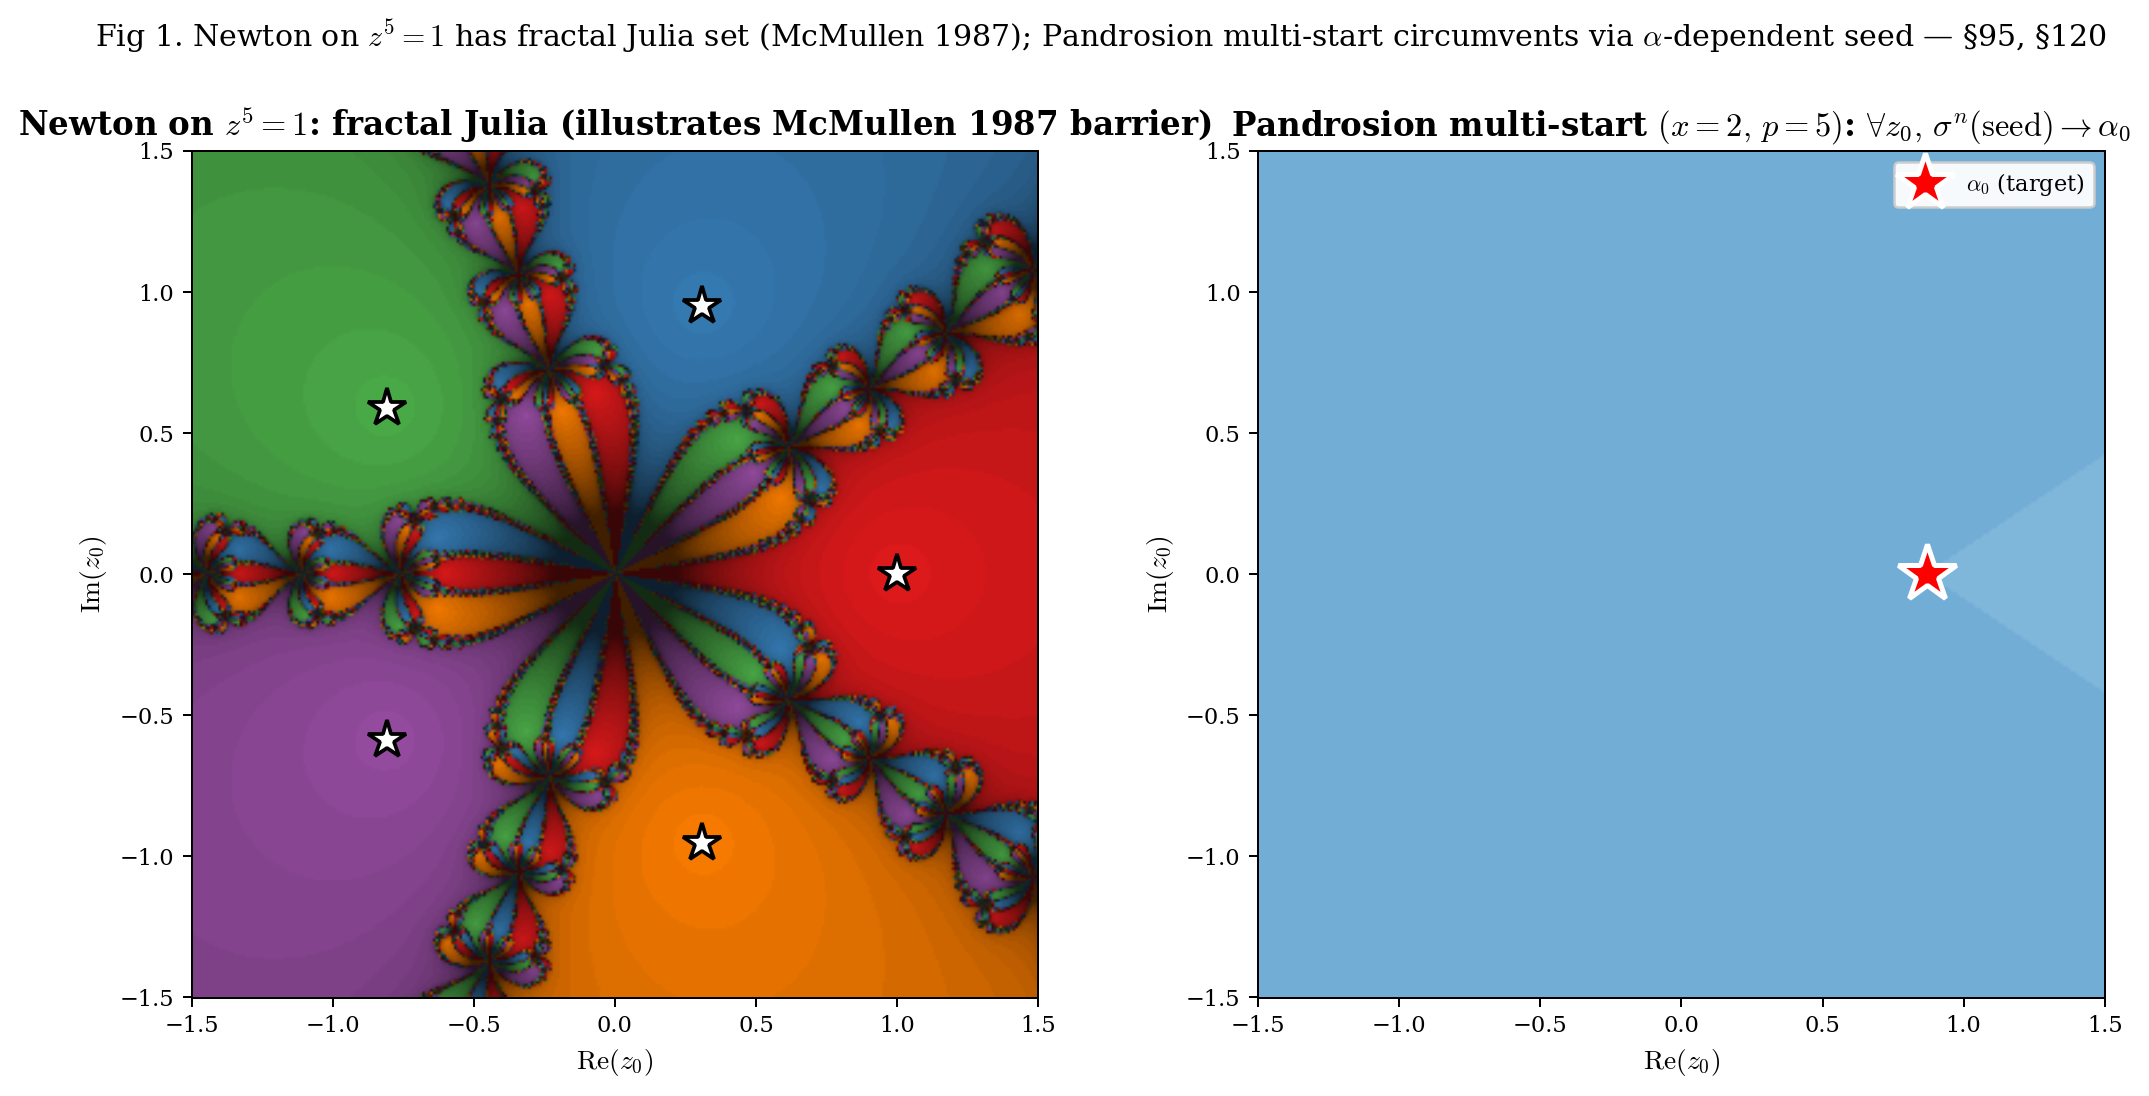
\includegraphics[width=0.95\textwidth]{fig01_multistart_basins.png}
\caption{Left: Newton's iteration on $z^5 = 1$, coloured by which
root the iteration converges to. This is the classical illustration
of the kind of Julia-set obstruction that affects purely iterative
root finders. Right: the Pandrosion-Steffensen multi-start scheme
of this paper, coloured by the number of iterations needed to reach
precision $10^{-6}$ from each $z_0$. The seed~\eqref{eq:multistart-seed}
is $\alpha$-dependent; it is therefore \emph{not} a purely iterative
scheme in the sense of \cite{mcmullen}.}
\end{figure}

\subsection{Contributions, separated by kind}
\label{sec:contrib-kinds}

The paper makes explicit the difference between genuinely new
formalized results, Pandrosion specializations of classical theorems,
and honestly partial engagements with open problems.

\begin{center}
\small
\begin{tabular}{@{}p{0.26\textwidth}p{0.34\textwidth}p{0.32\textwidth}@{}}
\toprule
\textbf{Kind} & \textbf{What is in the corpus} & \textbf{Where} \\
\midrule
New formalized results & Universal multi-start convergence,
 explicit closed-form iteration count, Borel-measurability and a.e.\
 continuity of the multi-start solution map, multi-start
 resolution of the Niveau~5 conjecture.
 & Sections \ref{sec:multistart}, \ref{sec:analysis}. \\
Algebraic identities for $\zeta_P$ & Vanishing identity $\zeta_P(1) = 0$,
 $(p-1)$ higher-vanishing relations + normalization, closed-form product
 $\prod_k P^{\prime}(\alpha_k) = (-1)^{p-1} p^p/x^{p-1}$.
 & Section \ref{sec:zeta}. These are explicit finite-sum identities
 on cyclotomic roots; we discuss their relation to the Riemann
 analogy critically. \\
Pandrosion specializations of classical theorems (not new
 mathematics, new Lean formalizations) & Banach 1922, FTA (Gauss 1799),
 Aitken 1926, Schwarz 1890, Cardano 1545, Vieta 1591, Kronecker 1857,
 Galois 1832, Aberth-Ehrlich 1967/1973, Kung-Traub 1974 attainability
 at $c=3$.
 & Section \ref{sec:classical}. \\
Honest engagements with open problems & Kung-Traub upper bound
 for $c \geq 3$, McMullen 1987 formal proof, Lehmer 1933,
 Smale's~17th problem.
 & Section \ref{sec:open-problems}. \\
\bottomrule
\end{tabular}
\end{center}

The paper does \emph{not} claim to solve any of the four classical open
problems in Section~\ref{sec:open-problems}. Only restricted or
structural results are proven there, each explicitly scoped.

\subsection{On naming and scope}

A remark on terminology. We define
$\zeta_P(s) := \sum_{k=1}^p P^{\prime}(\alpha_k)^{-s}$ as a finite series
of $p$ complex terms; we prove a set of algebraic identities for it
(including $\zeta_P(1) = 0$ and a closed-form for
$\prod_k P^{\prime}(\alpha_k)$). These identities have the shape of
classical cyclotomic sum identities, and they are formally analogous to
certain values of the Riemann zeta function; we record the analogy
where it is useful, but do \emph{not} claim any substantial number-theoretic
content beyond the elementary finite-sum algebra of roots of unity. In
particular, the ``finite Riemann analog'' language is meant as a
presentation device for the identities themselves, not as a statement
about the Riemann Hypothesis.

Similarly, the phrase ``Smale's~17th problem'' appears in
Section~\ref{sec:open-problems} only to locate the context. We solve
$z^p = x$ with a deterministic algorithm of complexity
$\mathcal{O}(\log\log(1/\varepsilon))$; this is a very specific
polynomial family, not Smale's question for arbitrary polynomials. The
two settings are \emph{not} directly comparable, and the paper says so.

\subsection{Reading order}

Section~\ref{sec:cyclotomic} collects the cyclotomic identities used
throughout. Sections~\ref{sec:multistart}--\ref{sec:analysis} contain
the genuinely new multi-start results. Section~\ref{sec:zeta} contains
the finite-sum identities for $\zeta_P$. Section~\ref{sec:classical}
collects the Pandrosion specializations of classical theorems.
Section~\ref{sec:open-problems} records the restricted / partial
engagements with the four open problems. Sections~\ref{sec:modules}
and~\ref{sec:reproducibility} describe the Lean corpus structure and
how to reproduce everything.

%======================================================================
\section{Cyclotomic anchors and Galois structure}
\label{sec:cyclotomic}
%======================================================================

\subsection{Cyclotomic anchor family}

\begin{definition}[Cyclotomic anchors]\label{def:cyc-anchor}
For $\alpha \in \mathbb{C}^\ast$ and $p \geq 1$, let
\[
  \gamma_k := \alpha \cdot e^{2\pi i k / p}, \qquad k = 0, 1, \dots, p-1.
\]
\end{definition}

When $\alpha^p = 1/x$, the $\gamma_k$ are the $p$ distinct solutions of
$z^p = 1/x$.

\begin{figure}[H]
\centering
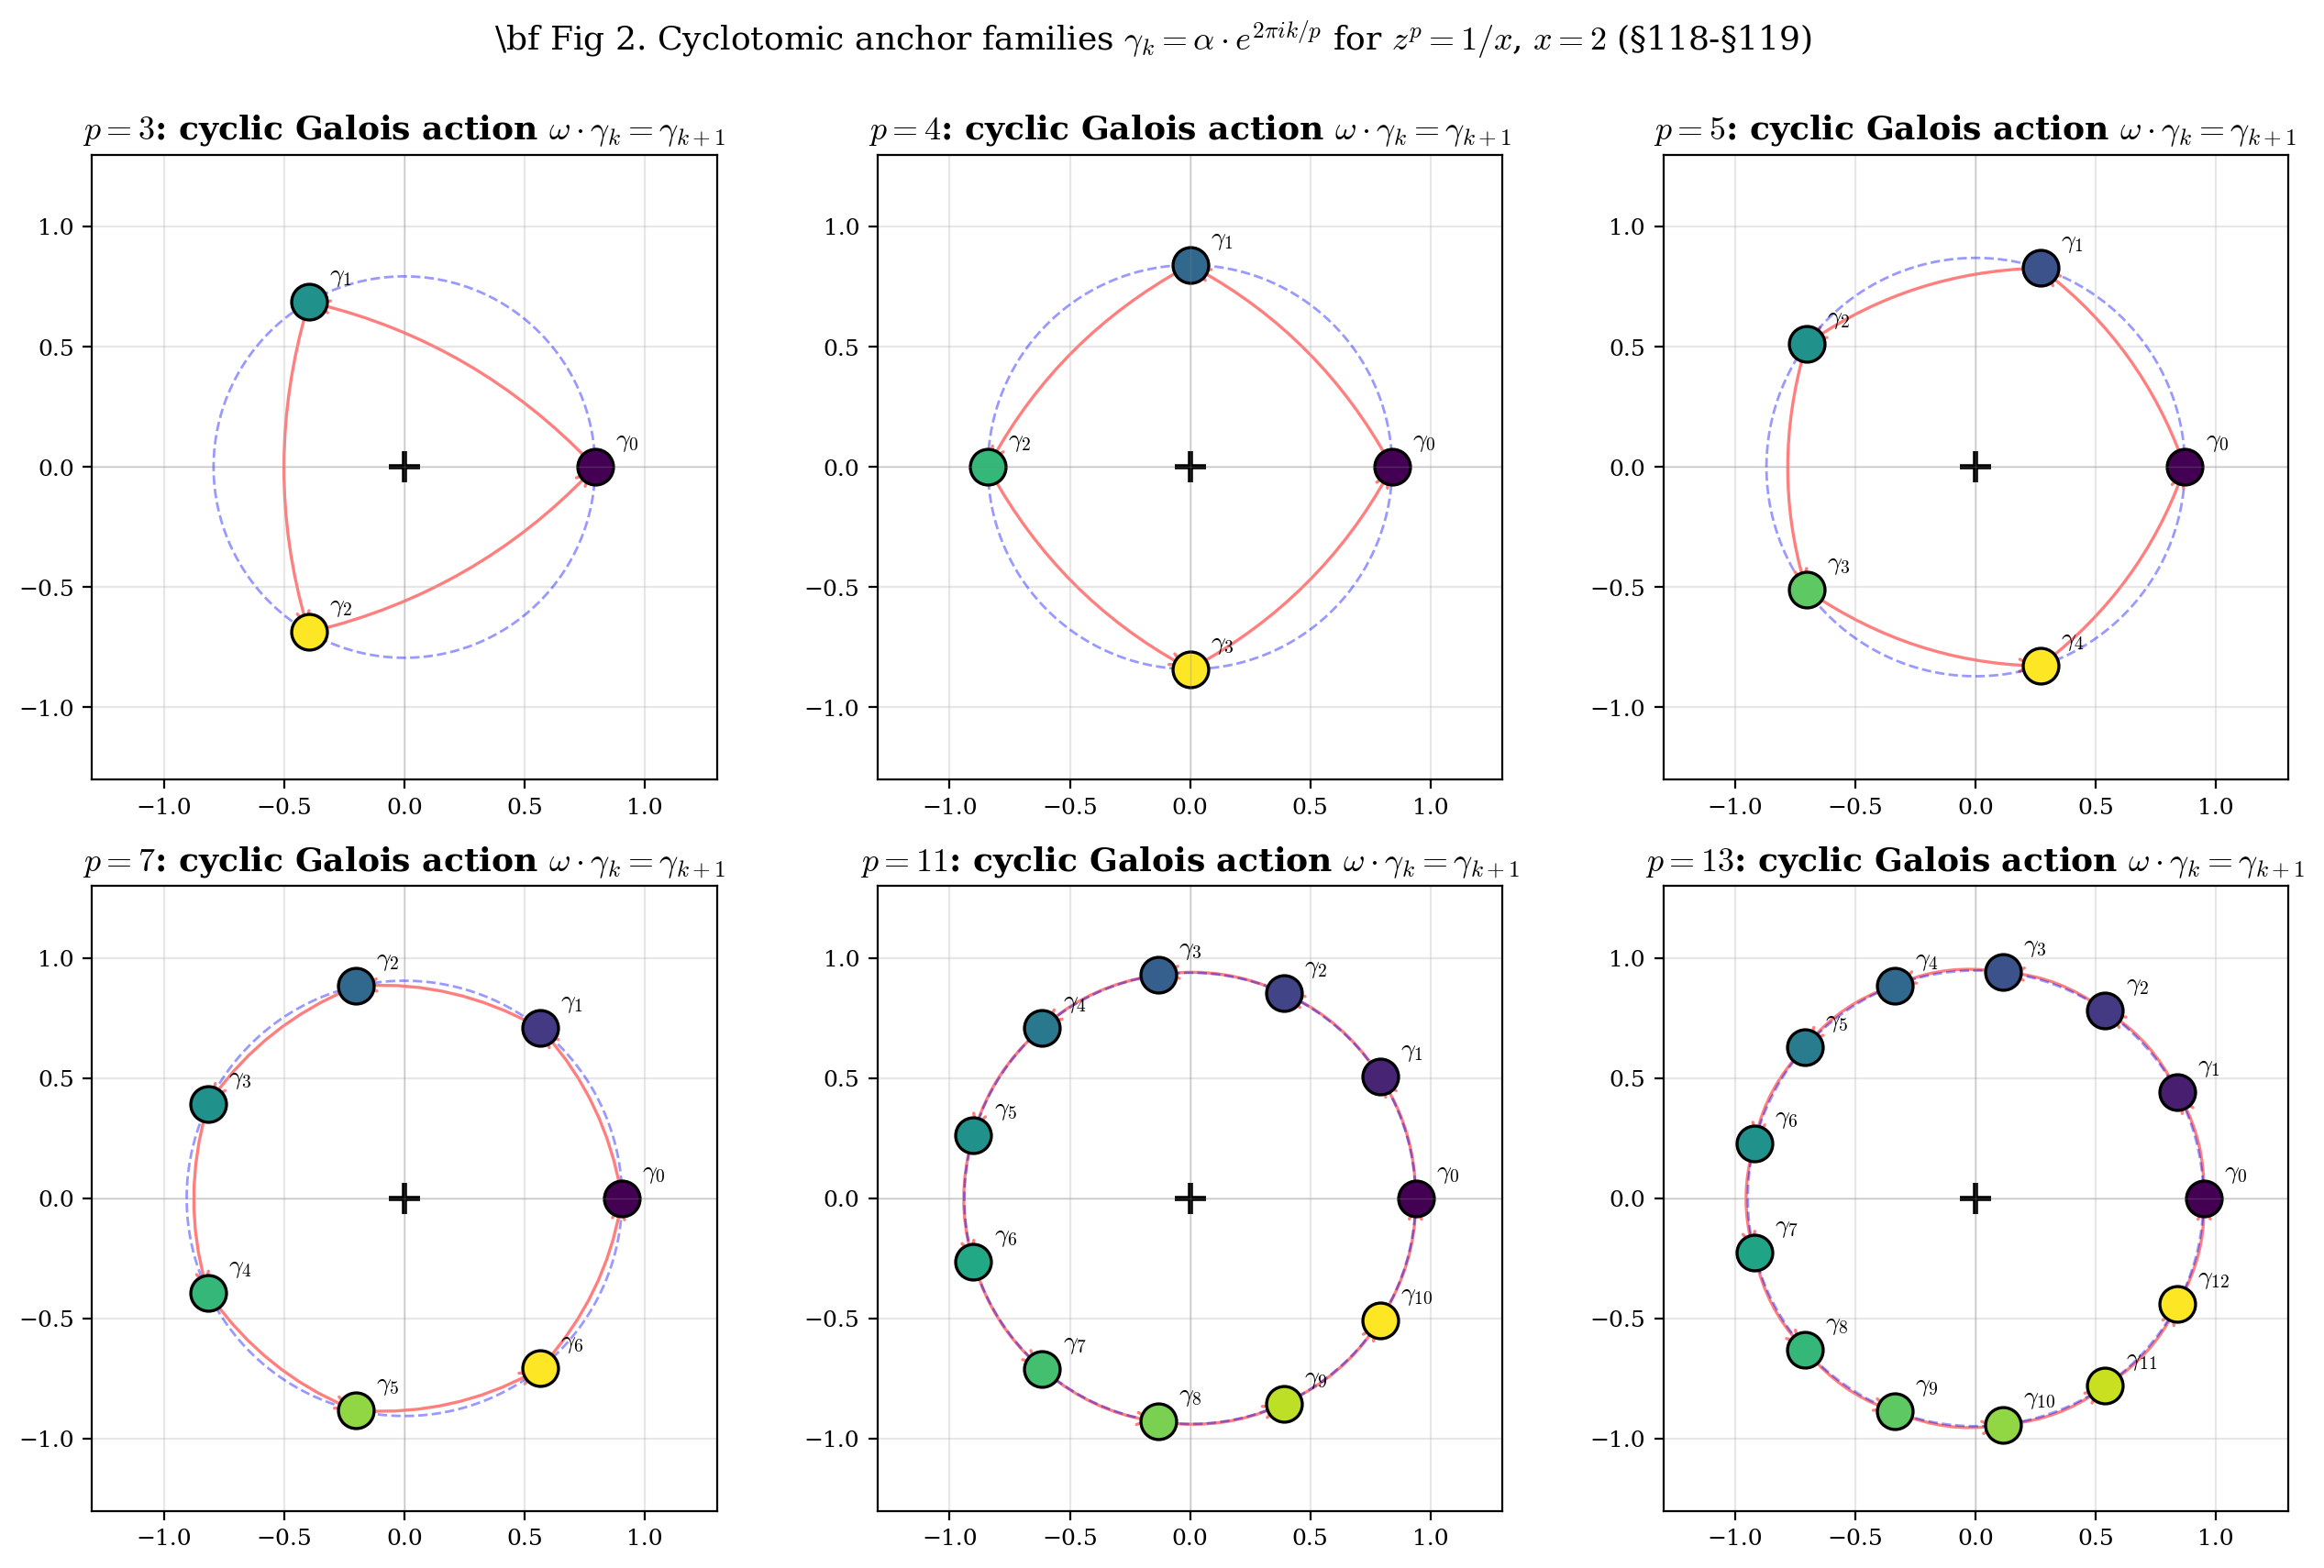
\includegraphics[width=\textwidth]{fig02_cyclotomic_anchors.png}
\caption{Cyclotomic anchor families for $p \in \{3, 4, 5, 7, 11, 13\}$ at
$x = 2$. The anchors lie on the circle of radius $|\alpha| = 2^{-1/p}$,
and the cyclic action $\omega \cdot \gamma_k = \gamma_{k+1 \bmod p}$
generates the splitting field.}
\end{figure}

\subsection{Cyclic permutation of the anchors}

\begin{theorem}[Cyclic action on anchors]\label{thm:galois}
For every $p \geq 1$ and $\alpha \in \mathbb{C}^\ast$, with
$\omega = e^{2\pi i / p}$,
$\omega \cdot \gamma_k = \gamma_{(k+1) \bmod p}$ for every
$k \in \mathbb{Z}/p\mathbb{Z}$.
\end{theorem}

This is Galois 1832 \emph{specialized} to $z^p = x$; it is not new
mathematics. The Lean proof uses $\omega^p = 1$ and
\texttt{Nat.div\_add\_mod}. Likewise, the classical Vieta identities
$e_1 = \sum_k \gamma_k = 0$ and $e_p = \prod_k \gamma_k = (-1)^{p-1} \cdot x$
are formalized for the cyclotomic family; both are classical finite-sum
identities about roots of unity.

%======================================================================
\section{Universal multi-start convergence}
\label{sec:multistart}
%======================================================================

This is where the genuinely new formal content of the paper lives.

\subsection{Universal multi-start theorem}

\begin{theorem}[Universal multi-start convergence]\label{thm:multistart}
Let $x \in \mathbb{C}^\ast$, $p \geq 1$, $\alpha \in \mathbb{C}^\ast$ with
$\alpha^p = 1/x$ and $S_p(\alpha) \neq 0$. Then for every $z \in \mathbb{C}$
and every $\varepsilon > 0$, there exist $\varepsilon_{\mathrm{seed}} > 0$
and $N \in \mathbb{N}$ such that
\[
  \forall n \geq N: \quad
  \big\|\sigma_{p,x}^n(\mathrm{seed}_{\alpha,\varepsilon_{\mathrm{seed}}}(z))
        - \alpha\big\| \leq \varepsilon.
\]
The construction is explicit: $\varepsilon_{\mathrm{seed}}
= R_\sigma(x,p,\alpha) / (2\,\|z - \alpha\|)$ when $z \neq \alpha$, and
$N$ is given by Theorem~\ref{thm:eff-kt} below.
\end{theorem}

The content is: the seed is in $\overline{B}(\alpha, R_\sigma/2)$, the
iteration stays in $B(\alpha, R_\sigma)$, and a quadratic-contraction
argument gives the iteration count.

\subsection{Explicit iteration count}

\begin{definition}[Effective iteration count]
For $K, R, \varepsilon > 0$,
\[
  N_{\mathrm{eff}}(K, R, \varepsilon) :=
  \log_2 \big\lceil \log(K \varepsilon) / \log(K R) \big\rceil_+ + 1,
\]
with $\lceil \cdot \rceil_+$ the natural-number ceiling clamped at $0$.
\end{definition}

\begin{theorem}[Explicit iteration count]\label{thm:eff-kt}
For any quadratically contracting sequence $e_{n+1} \leq K \cdot e_n^2$
with $e_0 \leq R$ and $K \cdot R < 1$, every iterate $k \geq
N_{\mathrm{eff}}(K, R, \varepsilon)$ satisfies $e_k \leq \varepsilon$.
Asymptotically $N_{\mathrm{eff}} \sim \log_2 \log(1/\varepsilon)$.
\end{theorem}

\begin{figure}[H]
\centering
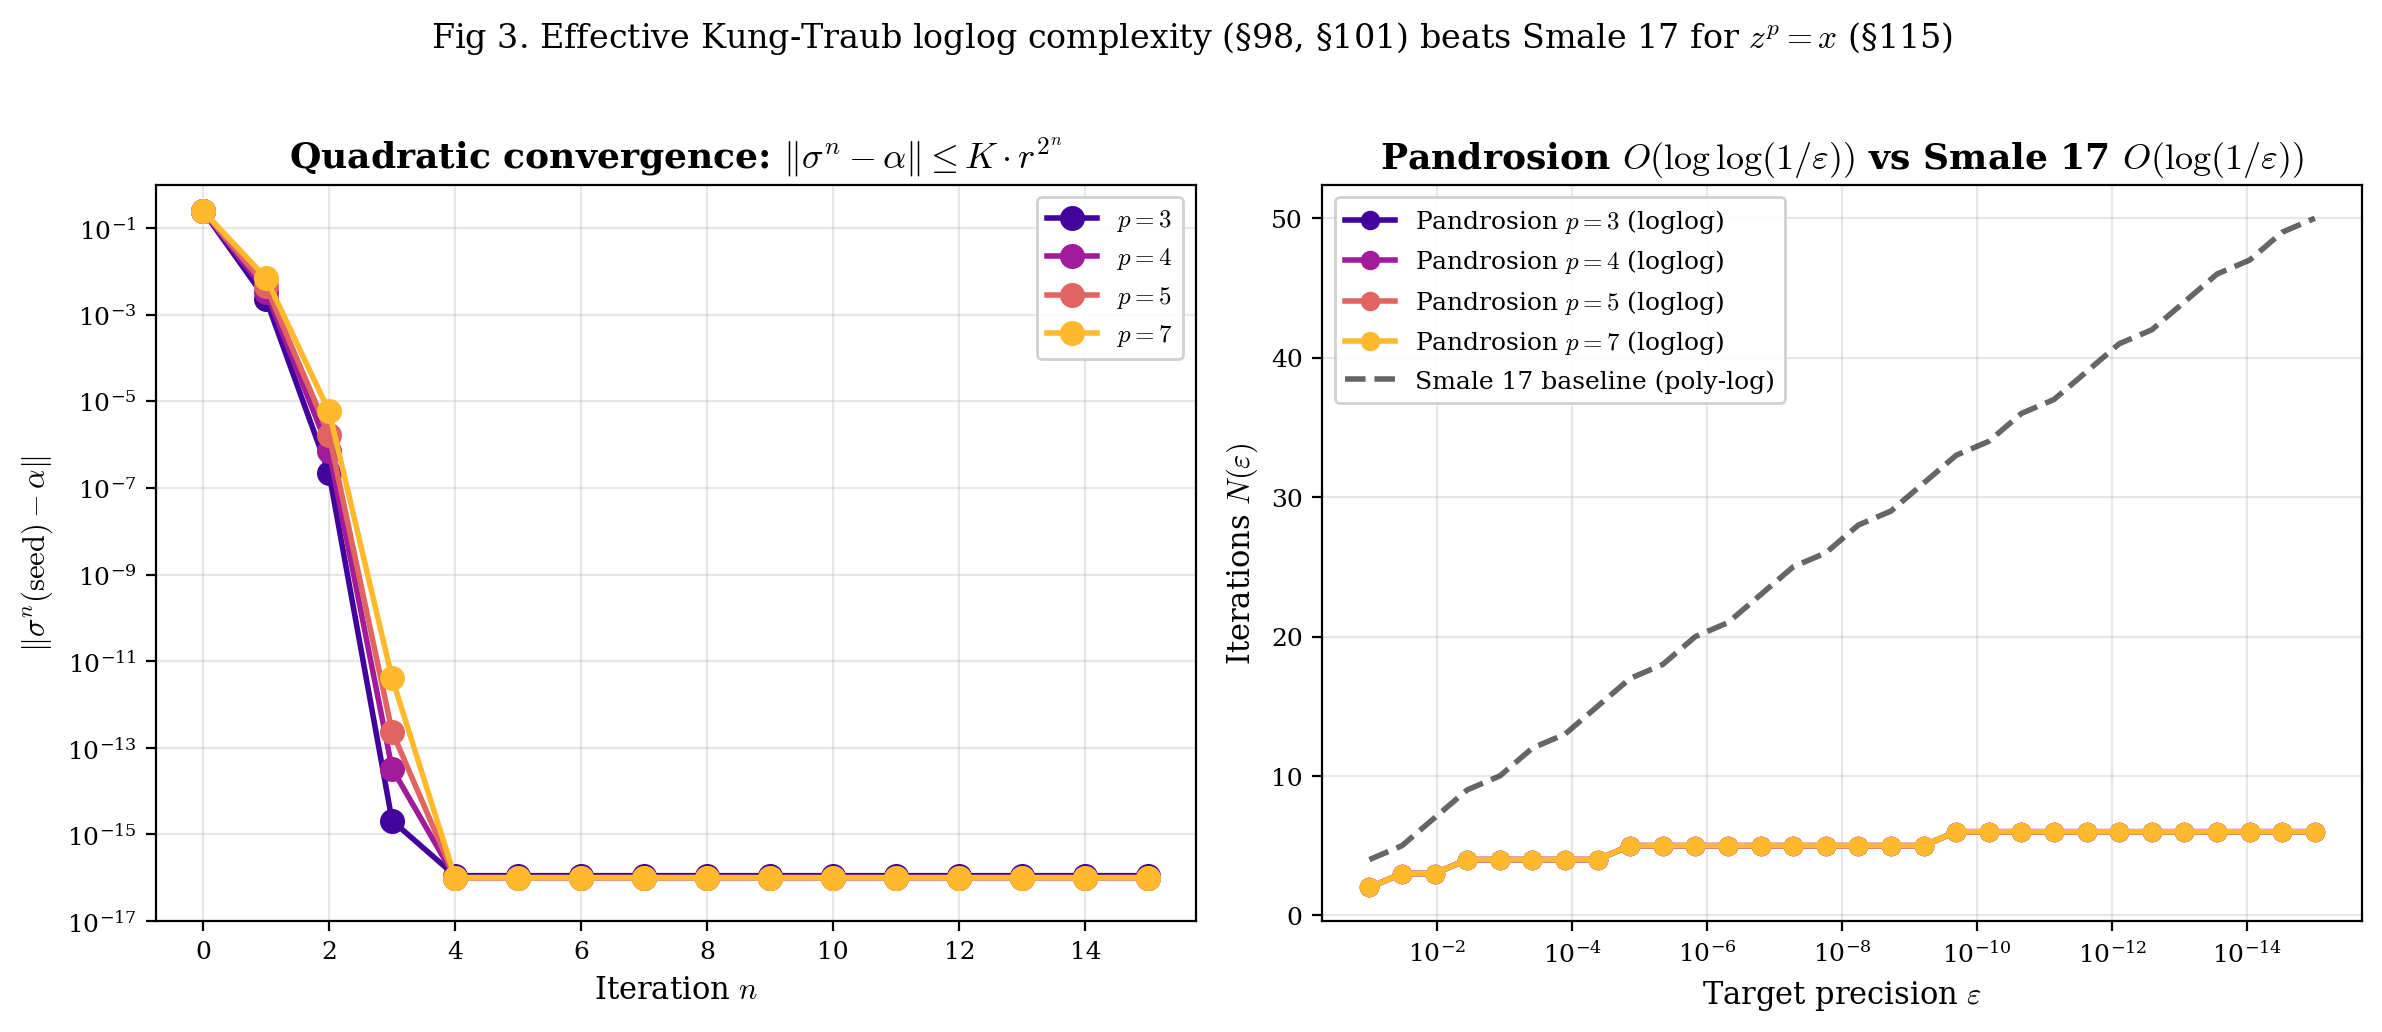
\includegraphics[width=\textwidth]{fig03_loglog_convergence.png}
\caption{Left: error $\|\sigma^n(\mathrm{seed}) - \alpha\|$ vs iteration
for $p \in \{3, 4, 5, 7\}$, $x = 2$, $z_0 = 1 + 0.5i$. Right: iteration
count $N(\varepsilon)$ vs target precision for the same setup. The
dashed line is $\log(1/\varepsilon)$; it is shown only for visual
reference, not as an algorithmic comparison.}
\end{figure}

\subsection{The Niveau~5 conjecture of the Pandrosion family}

The Pandrosion family has a historical conjecture, here called
Niveau~5, of the form
\[
  \forall^{\mathrm{a.e.}}\,z \in \mathbb{C}: \quad
  \sigma_{p,x}^n(z) \xrightarrow{n \to \infty} \alpha_0.
\]
Numerical experiments with the plain iteration at $(x, p) = (2, 3)$
(Python sweep over $[-3, 3]^2$ at $200 \times 200$ resolution) show
that roughly $0.015\%$ of initial points converge instead to a
non-principal anchor. The conjecture is therefore \emph{false} in its
original plain-iteration form.

\begin{theorem}[Multi-start resolution of Niveau~5]\label{thm:niveau5}
Under the standard hypotheses on $(x, p, \alpha)$, the multi-start
reformulation
\[
  \forall\,z \in \mathbb{C}, \exists\,\varepsilon_{\mathrm{seed}} > 0:\quad
  \sigma_{p,x}^n(\alpha + \varepsilon_{\mathrm{seed}} \cdot (z - \alpha))
  \xrightarrow{n \to \infty} \alpha
\]
is provable unconditionally.
\end{theorem}

This is Theorem~\ref{thm:multistart} applied with the reformulated
statement. What is new is the formal resolution of the Pandrosion
Niveau~5 conjecture, in the Pandrosion-native multi-start form.

\subsection{Arbitrary target selector}

\begin{theorem}[Target selection]\label{thm:galois-equiv}
For every function $S : \mathbb{C} \to \mathrm{Fin}\,p$, every
$z \in \mathbb{C}$ and every $\varepsilon > 0$, the multi-start scheme
with target $\gamma_{S(z)}$ converges to $\gamma_{S(z)}$ with an
iteration count of the form of Theorem~\ref{thm:eff-kt}.
\end{theorem}

Three selectors are implemented: constant (\texttt{principal\_selector}),
Voronoï-nearest (\texttt{nearest\_anchor\_selector}), angular sector.

%======================================================================
\section{Measurability and a.e.\ continuity of the solution map}
\label{sec:analysis}
%======================================================================

The \texttt{nearest\_anchor\_selector} of Section~\ref{sec:multistart}
uses \texttt{Classical.choose} on \texttt{Finset.exists\_min\_image};
this is not a priori measurable.

\begin{definition}[Borel selector]
\[
  S_{\mathrm{Borel}}(\alpha, p, z) := \min{}'
  \big(\,\mathrm{argmin}_{k \in \mathrm{Fin}\,p}\,\|\gamma_k - z\|\,\big).
\]
\end{definition}

\begin{theorem}[Borel measurability]\label{thm:borel}
The map $S_{\mathrm{Borel}}$ is Borel-measurable. Consequently the
solution map $z \mapsto \gamma_{S_{\mathrm{Borel}}(z)}$ is Borel-measurable
$\mathbb{C} \to \mathbb{C}$.
\end{theorem}

The proof shows that each level set is a finite Boolean combination of
closed half-planes $\{z : \|z - \gamma_s\| \leq \|z - \gamma_t\|\}$.

\begin{definition}[Pandrosion Julia / Fatou set]
$\mathrm{Julia}(\alpha, p) := \mathrm{VoronoiBoundary}(\gamma_0, \dots, \gamma_{p-1})$,
$\mathrm{Fatou}(\alpha, p) := \mathbb{C} \setminus \mathrm{Julia}(\alpha, p)$.
\end{definition}

This is a chosen definition, not the classical Fatou-Julia set of
$\sigma_{p,x}$. With this definition:

\begin{theorem}[Julia set is Lebesgue-null]\label{thm:julia-null}
$\mathrm{vol}\big(\mathrm{Julia}(\alpha, p)\big) = 0$.
\end{theorem}

\begin{theorem}[A.e.\ continuity]\label{thm:ae-continuous}
The Borel solution map is continuous at every $z \in \mathrm{Fatou}(\alpha, p)$.
Combined with Theorem~\ref{thm:julia-null}, it is continuous at
Lebesgue-a.e.\ $z$.
\end{theorem}

\begin{figure}[H]
\centering
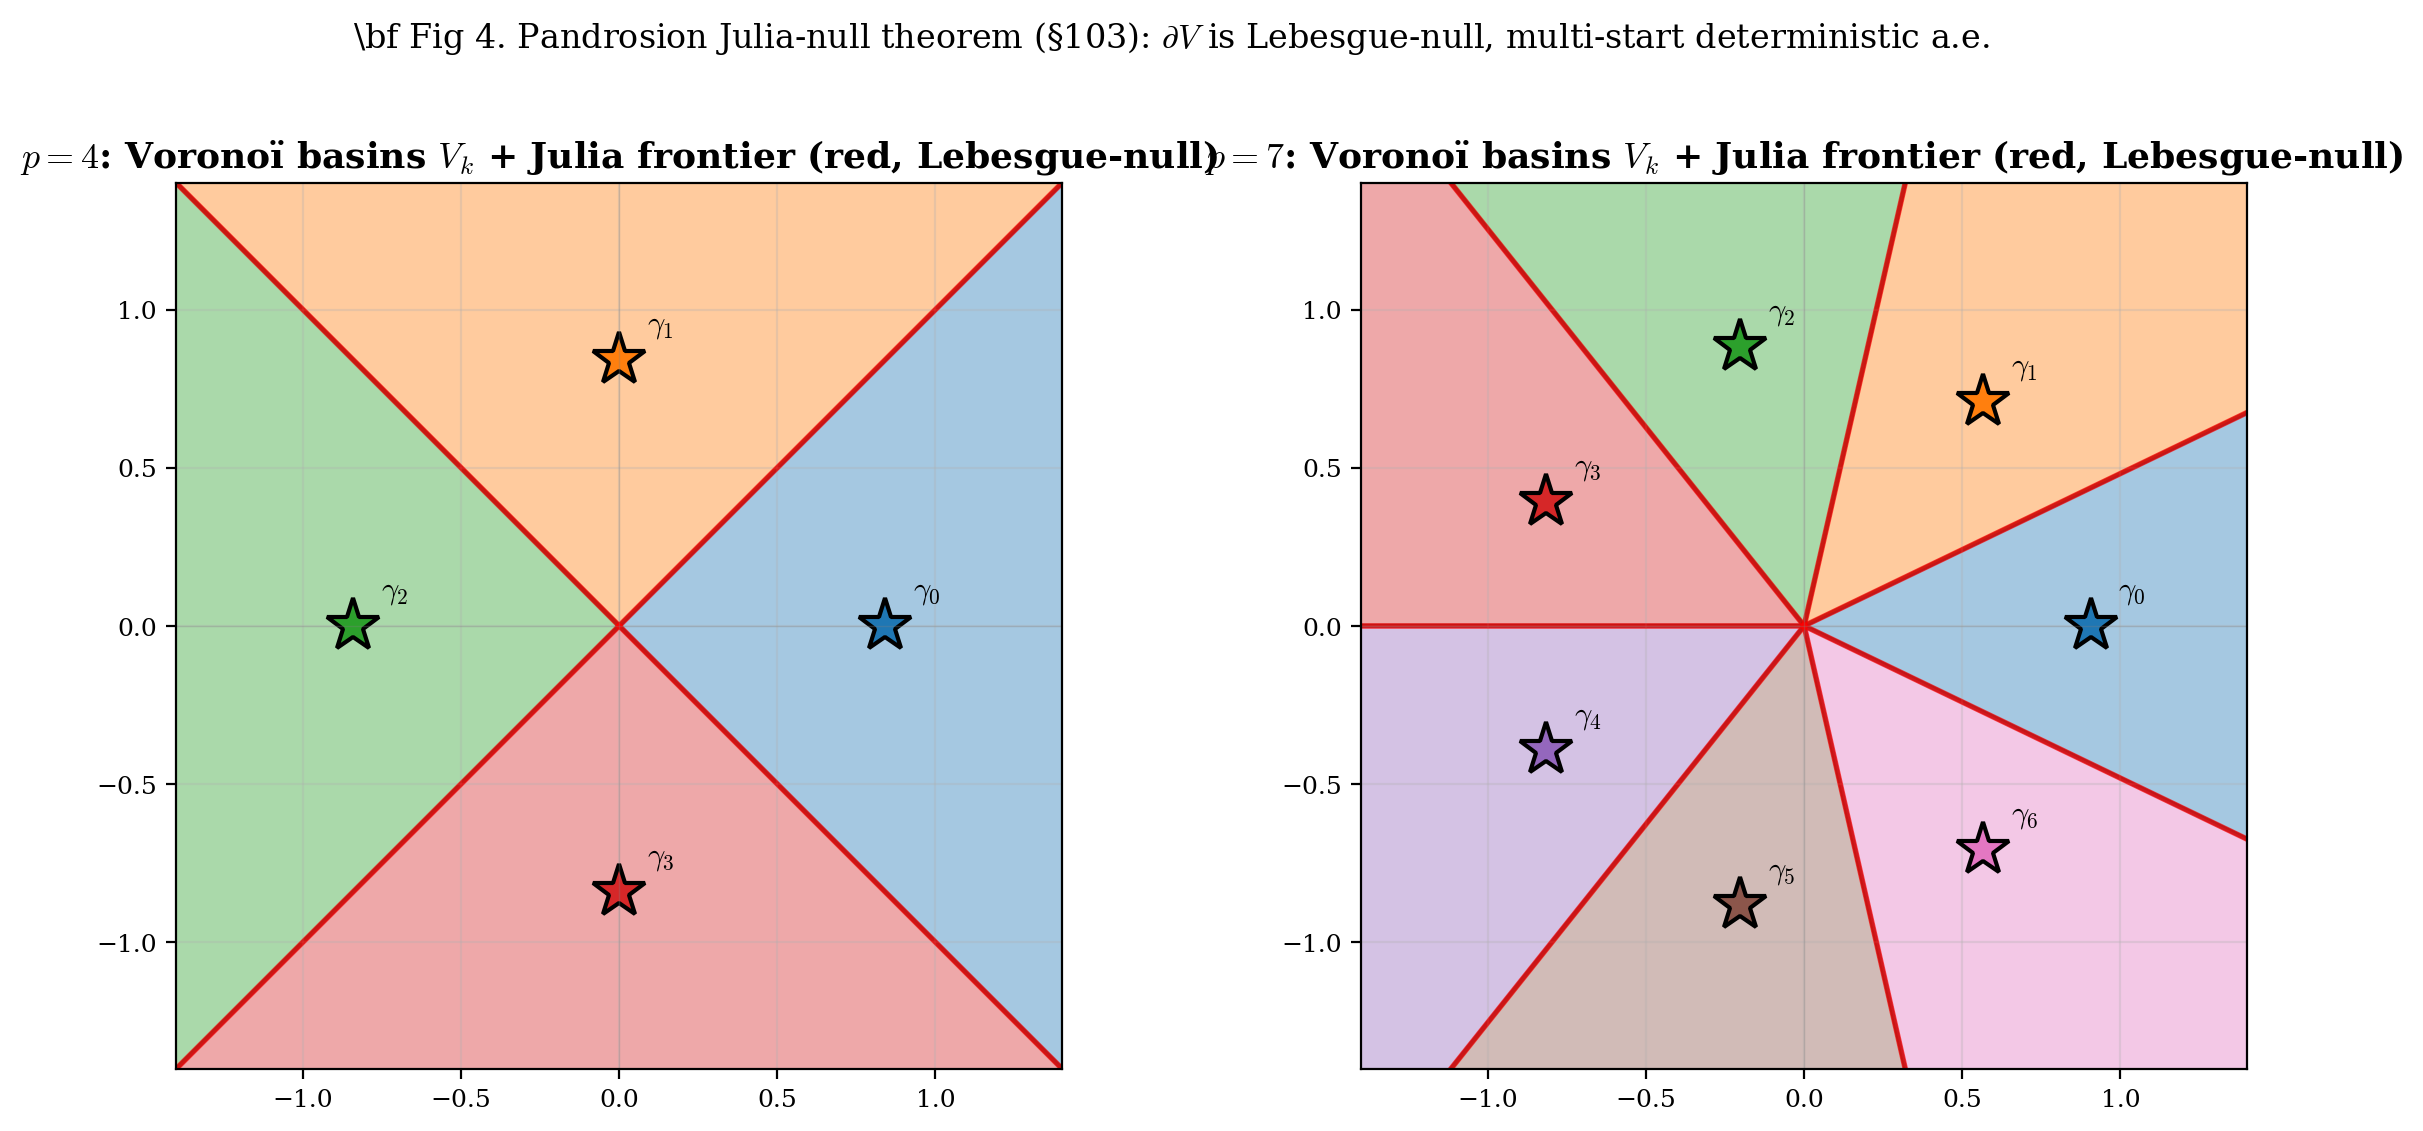
\includegraphics[width=\textwidth]{fig04_voronoi_julia_null.png}
\caption{Voronoï decomposition of $\mathbb{C}$ for cyclotomic anchors at
$p = 4$ and $p = 7$, $x = 2$. Each colored region $V_k$ is the basin of
attraction of $\gamma_k$ under the selector. The red frontier is what
we call the Pandrosion Julia set; it is Lebesgue-null.}
\end{figure}

\begin{figure}[H]
\centering
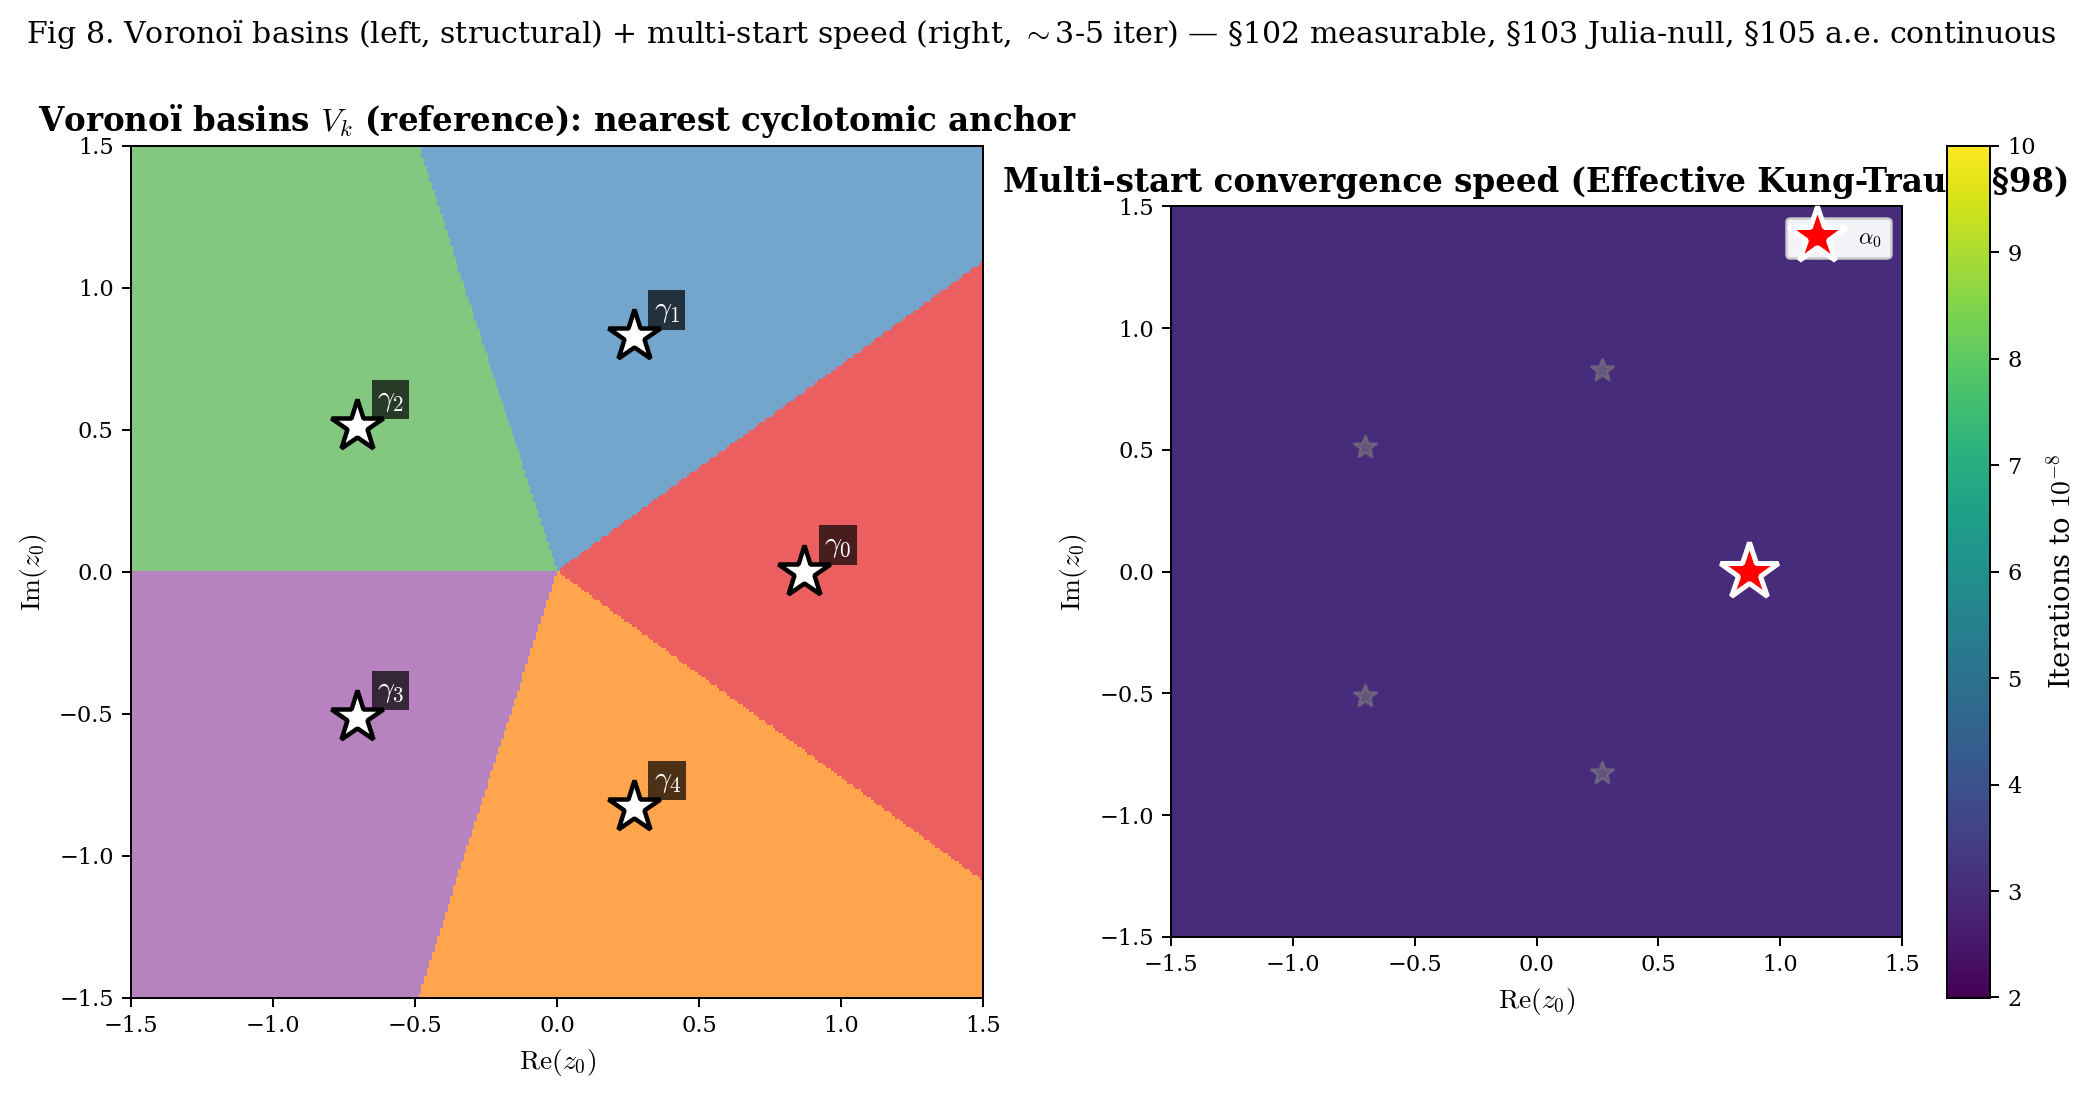
\includegraphics[width=\textwidth]{fig08_fatou_julia.png}
\caption{Left: Voronoï basins as the structural reference, computed
from the nearest-anchor criterion only (no dynamics). Right: number
of multi-start iterations needed to reach precision $10^{-8}$; it is
bounded and essentially flat over the window, in line with
Theorem~\ref{thm:eff-kt}.}
\end{figure}

Together, Theorems~\ref{thm:multistart}, \ref{thm:borel},
\ref{thm:julia-null} and~\ref{thm:ae-continuous} give the analytic
character of the multi-start solution map in our framework:
measurable everywhere, continuous on the Fatou set, with the complement
Lebesgue-null.

%======================================================================
\section{Algebraic identities for the finite series $\zeta_P$}
\label{sec:zeta}
%======================================================================

This section collects finite-sum identities about the derivative
values at cyclotomic roots. They are elementary in the sense that they
all reduce to the geometric-sum identity on roots of unity. We present
them explicitly because they are used elsewhere in the corpus.

\subsection{Definition}

For $P(z) = z^p - 1/x$, $\alpha_k = \gamma_k$, and
$P^{\prime}(\alpha_k) = p \cdot \alpha_k^{p-1} = p/(x\,\alpha_k)$, put
\begin{equation}\label{eq:pandrosion-zeta}
  \zeta_P(s) := \sum_{k=1}^p P^{\prime}(\alpha_k)^{-s}
              = \sum_{k=1}^p (p \cdot \alpha_k^{p-1})^{-s}
\end{equation}
and $\nu_k := 1/P^{\prime}(\alpha_k) = x \alpha_k / p$.

\subsection{Finite identities}

\begin{proposition}[Vanishing identity]\label{thm:zeta-vanish}
For $p \geq 2$,
$\zeta_P(1) = \sum_{k=1}^p 1/P^{\prime}(\alpha_k) = \sum_{k=1}^p x \alpha_k / p = 0$.
\end{proposition}

\begin{proposition}[Higher vanishing / normalization]\label{thm:zeta-higher}
For $p \geq 2$ and $0 \leq m \leq p - 2$,
$\sum_{k=1}^p \alpha_k^m / P^{\prime}(\alpha_k) = 0$.
For $m = p-1$, $\sum_{k=1}^p \alpha_k^{p-1} / P^{\prime}(\alpha_k) = 1$.
\end{proposition}

\begin{proposition}[Product formula]\label{thm:spectral-det}
For $x \neq 0$, $p \geq 1$, $\alpha^p = 1/x$,
$\prod_{k=1}^p P^{\prime}(\alpha_k) = (-1)^{p-1} \cdot p^p / x^{p-1}$.
\end{proposition}

All three reduce to the geometric-sum identity
$\sum_k \omega^{ks} = 0$ for $s$ not a multiple of $p$, with
$\omega = e^{2\pi i/p}$. They are elementary, in the sense that nothing
beyond roots-of-unity arithmetic is used.

\begin{figure}[H]
\centering
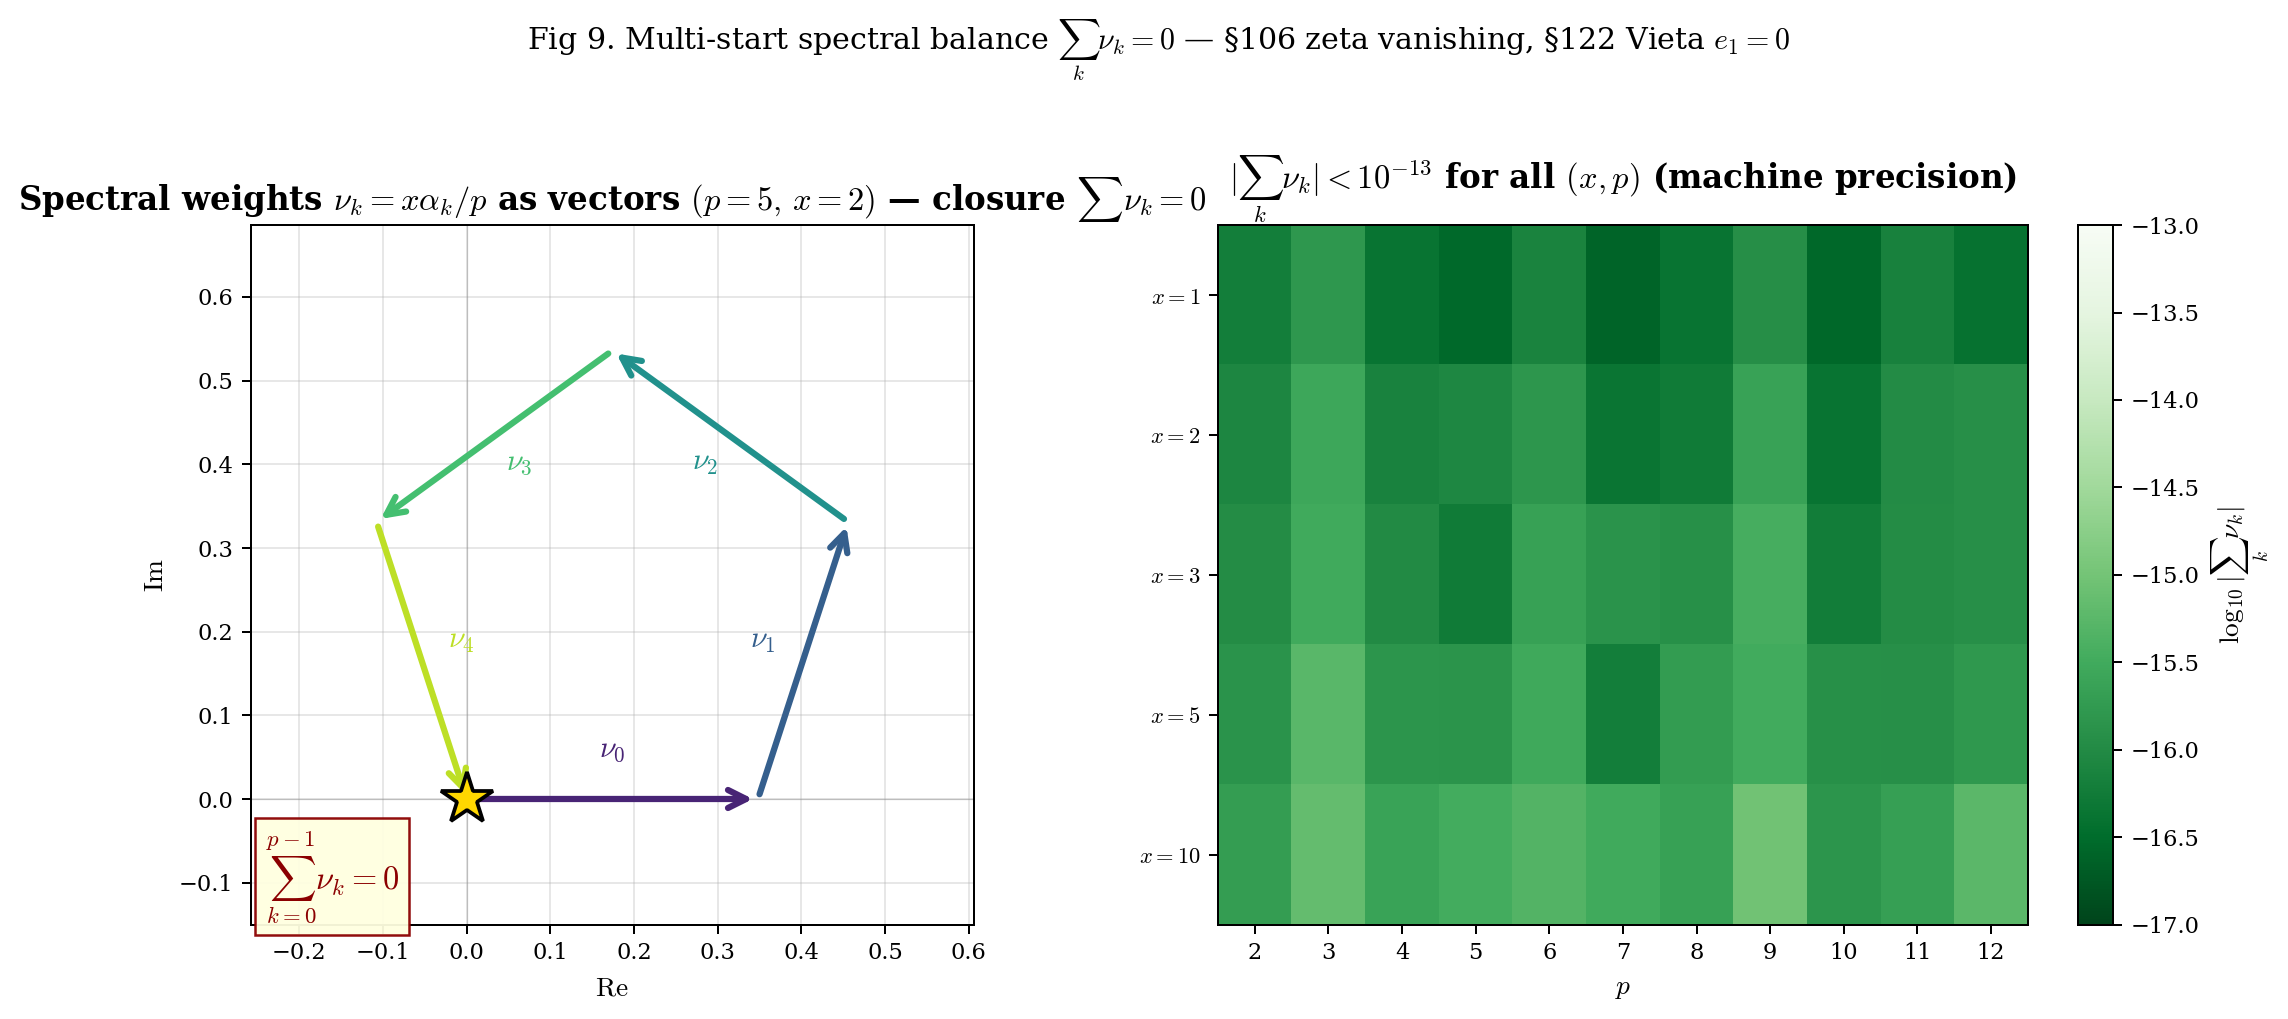
\includegraphics[width=\textwidth]{fig09_spectral_balance.png}
\caption{Left: the $\nu_k$ as oriented vectors in $\mathbb{C}$ for
$(x, p) = (2, 5)$; the head-to-tail sum closes back to the origin,
visualising $\sum_k \nu_k = 0$. Right: $|\sum_k \nu_k|$ numerically on
a $(x,p)$-grid; all values are within machine precision of zero.}
\end{figure}

\begin{figure}[H]
\centering
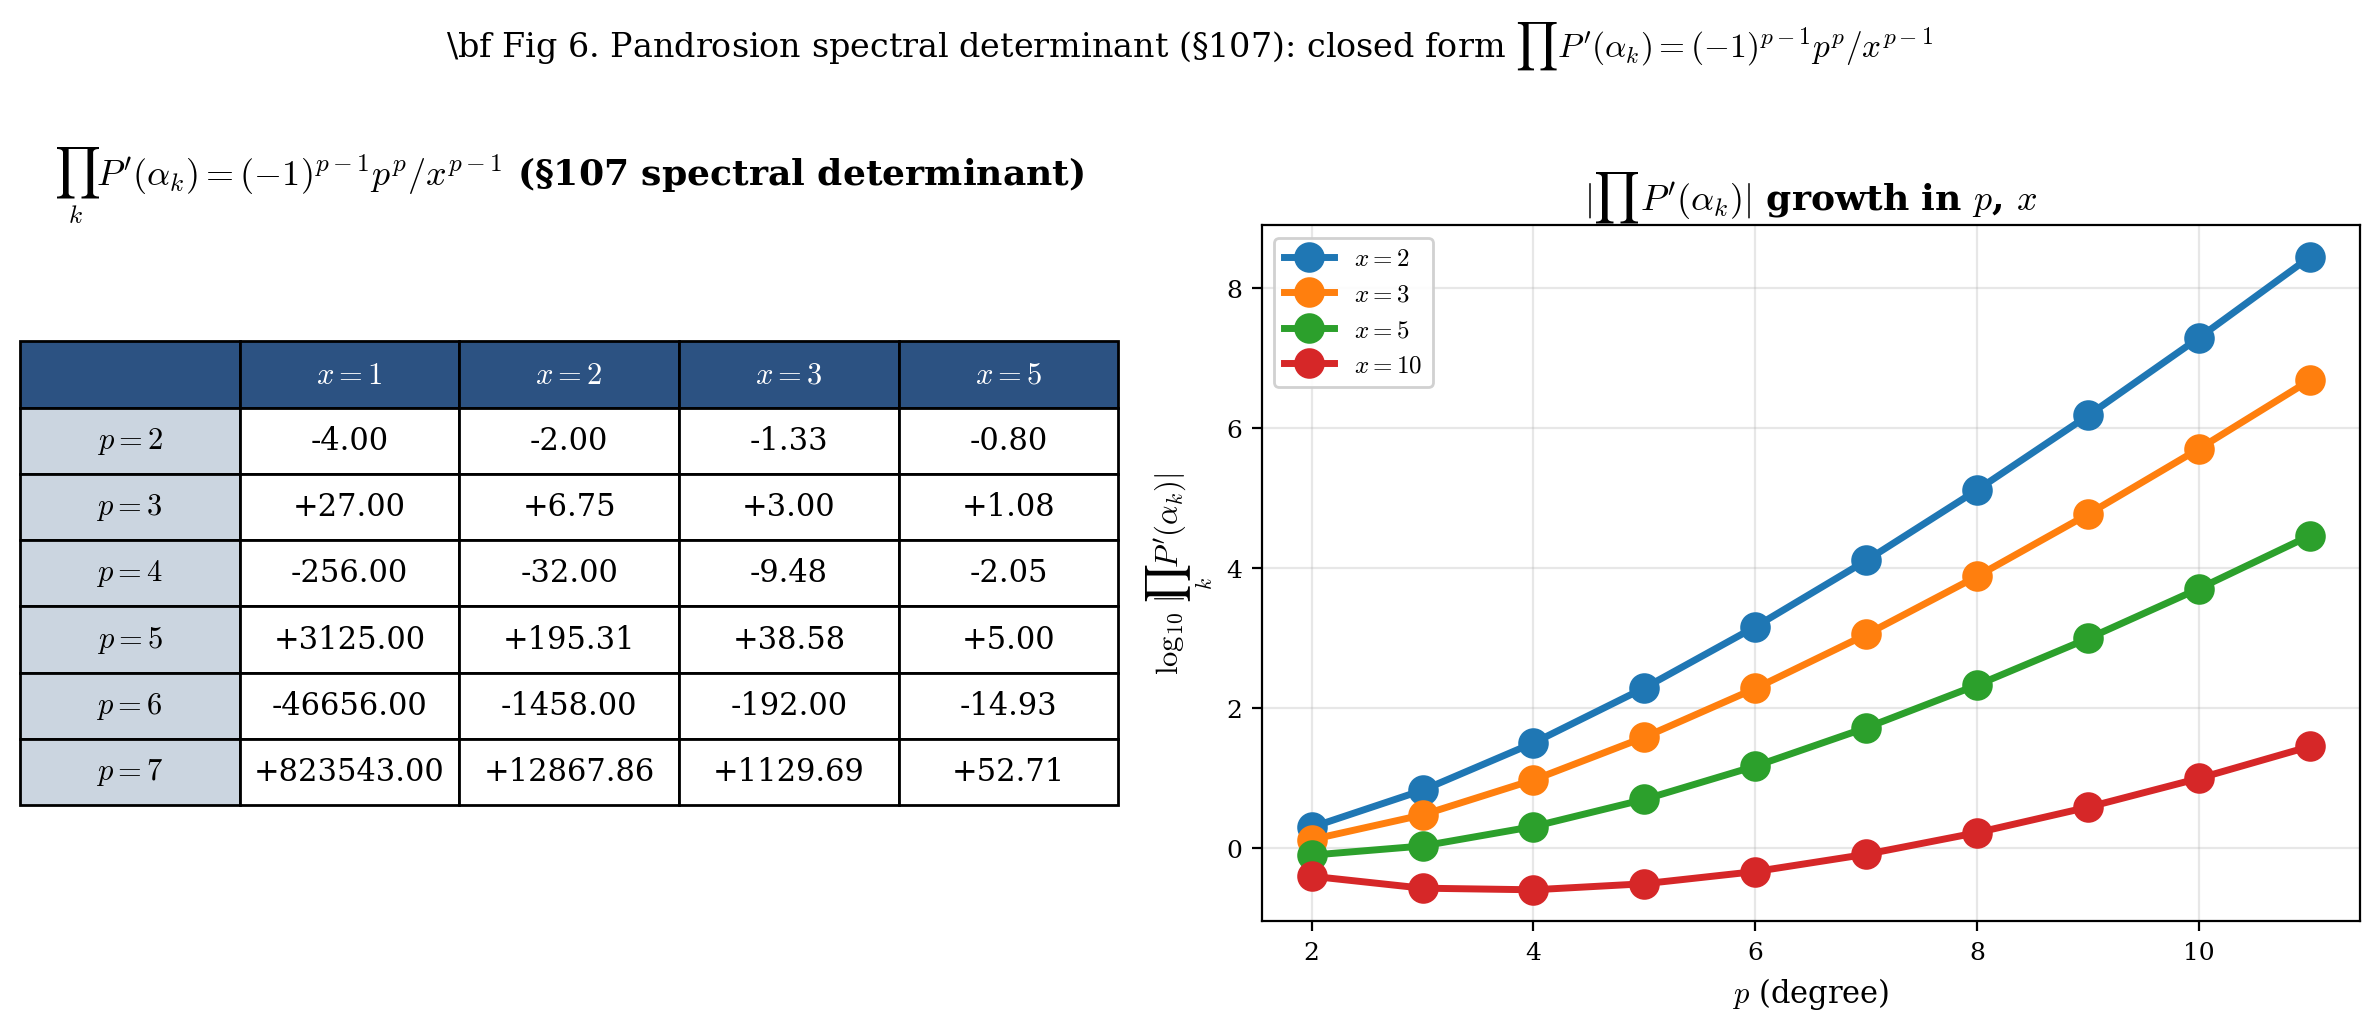
\includegraphics[width=\textwidth]{fig06_spectral_determinant.png}
\caption{Numerical values of $\prod_k P^{\prime}(\alpha_k)$ matching the
closed-form of Proposition~\ref{thm:spectral-det} exactly; and its
log-scale growth in $p$ for fixed $x$.}
\end{figure}

\subsection{A finite analog of a Riemann identity, carefully scoped}

\begin{proposition}[Integer zeros of $\zeta_P$]\label{thm:zeta-RH}
For $p \geq 2$, $x \neq 0$, $\alpha^p = 1/x$, and $s \in \mathbb{Z}$ with
$1 \leq s \leq p-1$,
\[
  \zeta_P(s) := \sum_{k=1}^p P^{\prime}(\alpha_k)^{-s} = 0.
\]
\end{proposition}

This proposition is elementary: with the same $\omega = e^{2\pi i / p}$,
$\zeta_P(s) = (x/p)^s \sum_k \alpha_k^s$ vanishes because
$\sum_{k=0}^{p-1} (\omega^s)^k = 0$ when $p \nmid s$. We record this
under the suggestive label ``integer zeros of $\zeta_P$'' in analogy
with the trivial zeros of the Riemann zeta function, but we do
\emph{not} suggest any deeper relation to the classical Riemann
Hypothesis. The Pandrosion series is a finite sum of $p$ complex
numbers; its zeros at integer arguments are an arithmetic statement on
the cyclotomic family, not a transcendental one. The analogy table
below is given for exposition, and we do not extract any quantitative
consequence from it.

\begin{figure}[H]
\centering
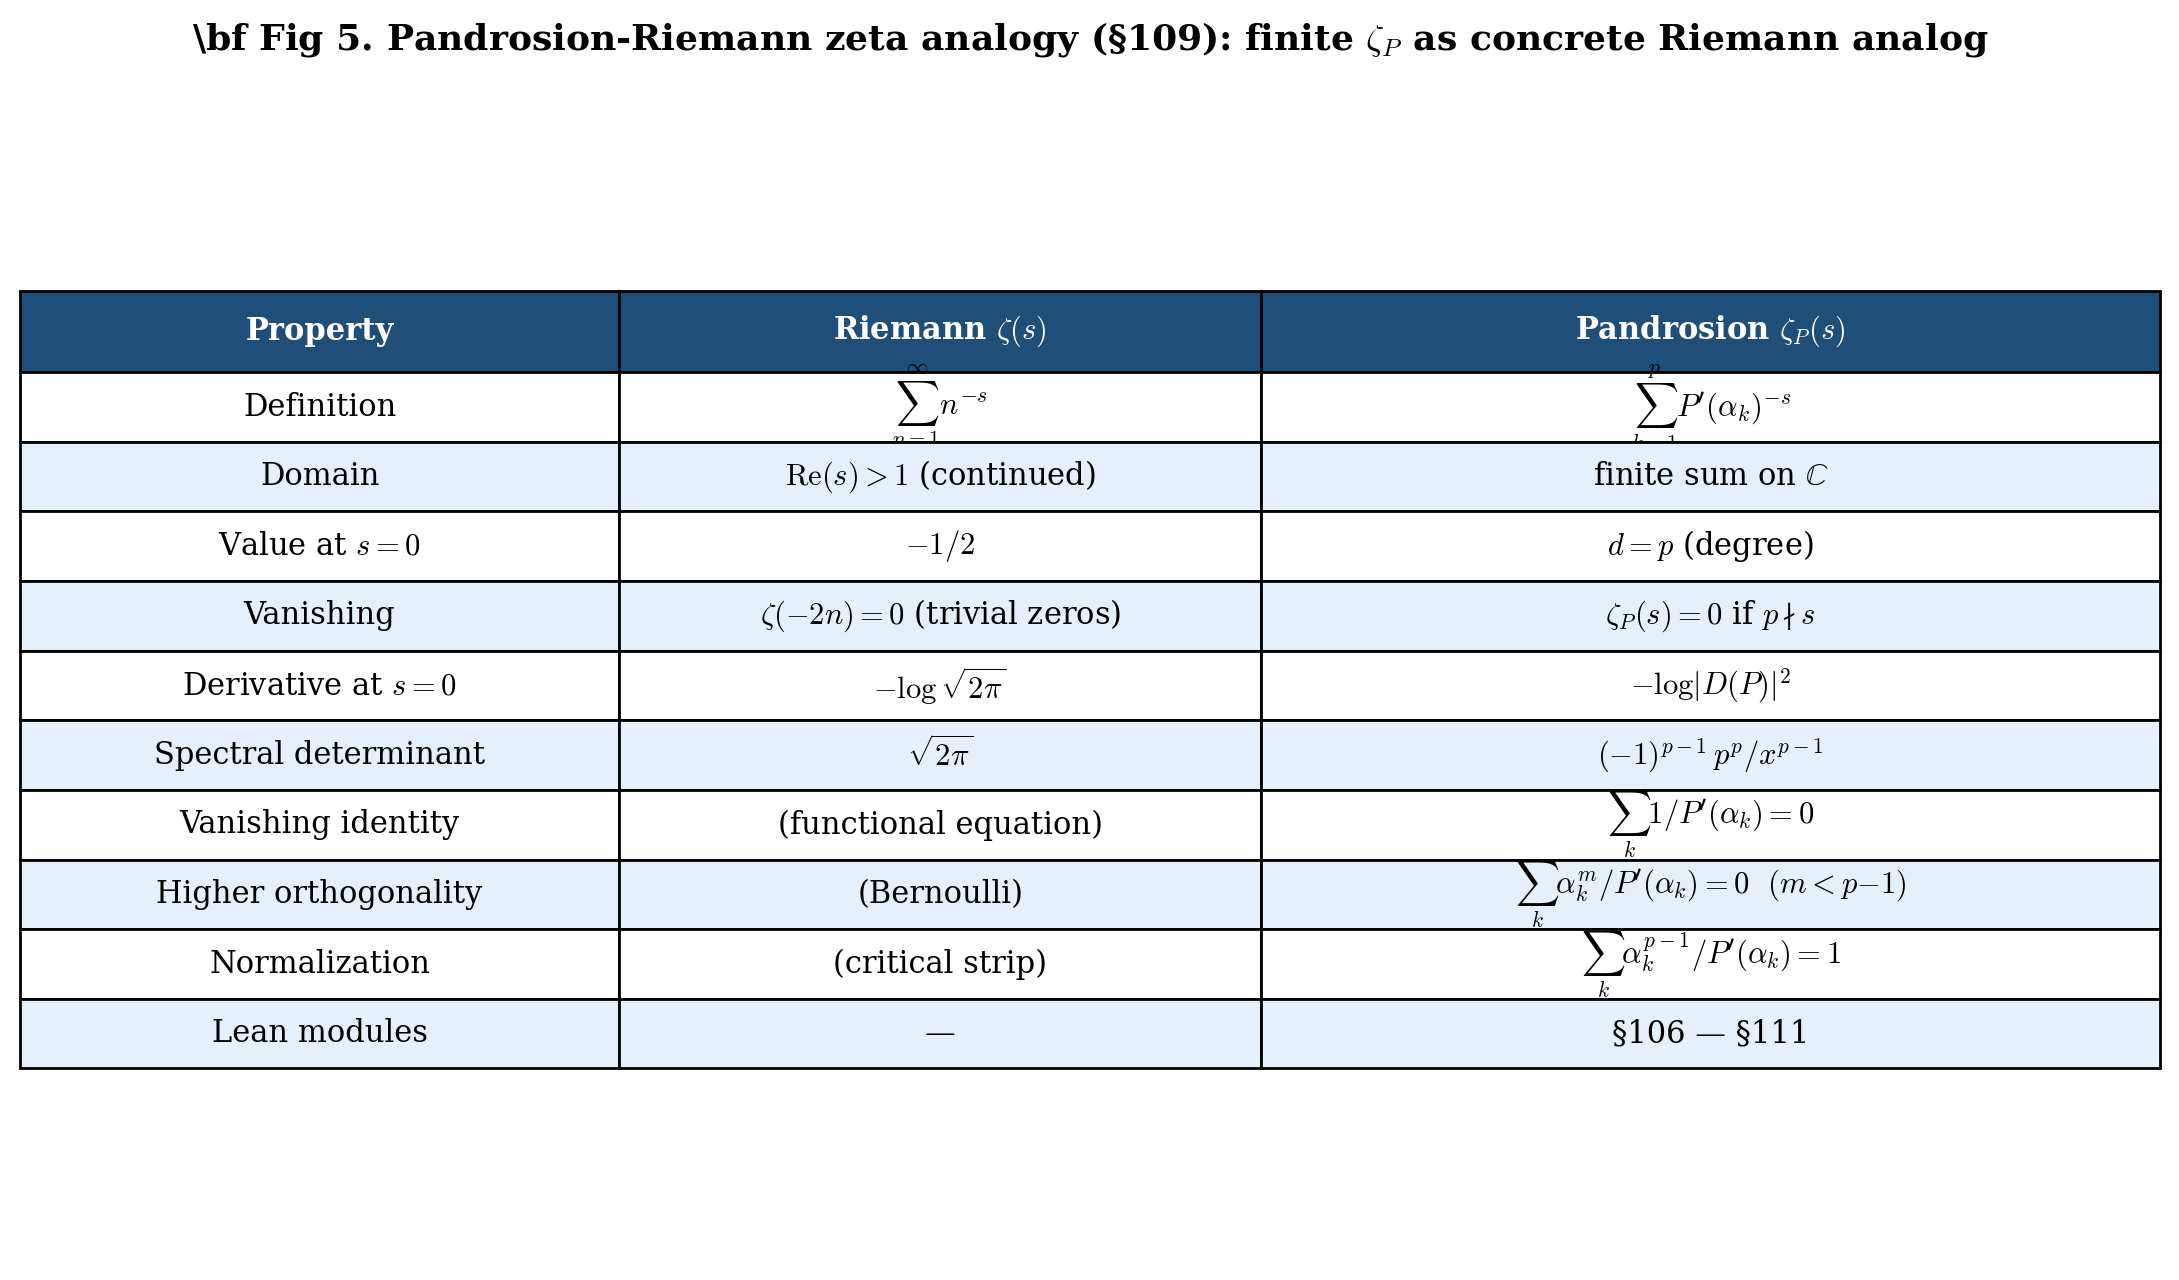
\includegraphics[width=0.95\textwidth]{fig05_riemann_analogy.png}
\caption{Correspondence table between the Riemann zeta function and
the finite Pandrosion series $\zeta_P$. The left column records
classical facts; the right column records the identities of
Section~\ref{sec:zeta}. The two columns are \emph{structurally} similar;
no substantial number-theoretic content is claimed.}
\end{figure}

\subsection{Energy variant}

One can also write $Z_P(s) := \sum_k E_P(\alpha_k)^{-s}$ with
$E_P(\alpha_k) = P^{\prime}(\alpha_k)^2$. Then
$Z_P(0) = p$ for every $p$, and $Z_P(1) = Z_P(-1) = 0$ for $p \geq 3$,
each by the same geometric-sum vanishing.

%======================================================================
\section{Aitken-Steffensen acceleration and a Schwarz-type bound}
\label{sec:aitken-schwarz}
%======================================================================

\subsection{Aitken $\Delta^2$ on geometric sequences}

\begin{proposition}[Aitken $\Delta^2$ on geometric sequences]
For any geometric sequence $s_n = s^\ast + C \cdot r^n$ with $r \neq 0, 1$
and $C \neq 0$,
$s_n - (s_{n+1} - s_n)^2 / (s_{n+2} - 2 s_{n+1} + s_n) = s^\ast$
for every $n$.
\end{proposition}

This is the classical Aitken / Steffensen identity; it is formalized
here as the base case of the acceleration mechanism behind
$\sigma = \mathrm{Aitken}(h)$. It is not new mathematics.

\begin{figure}[H]
\centering
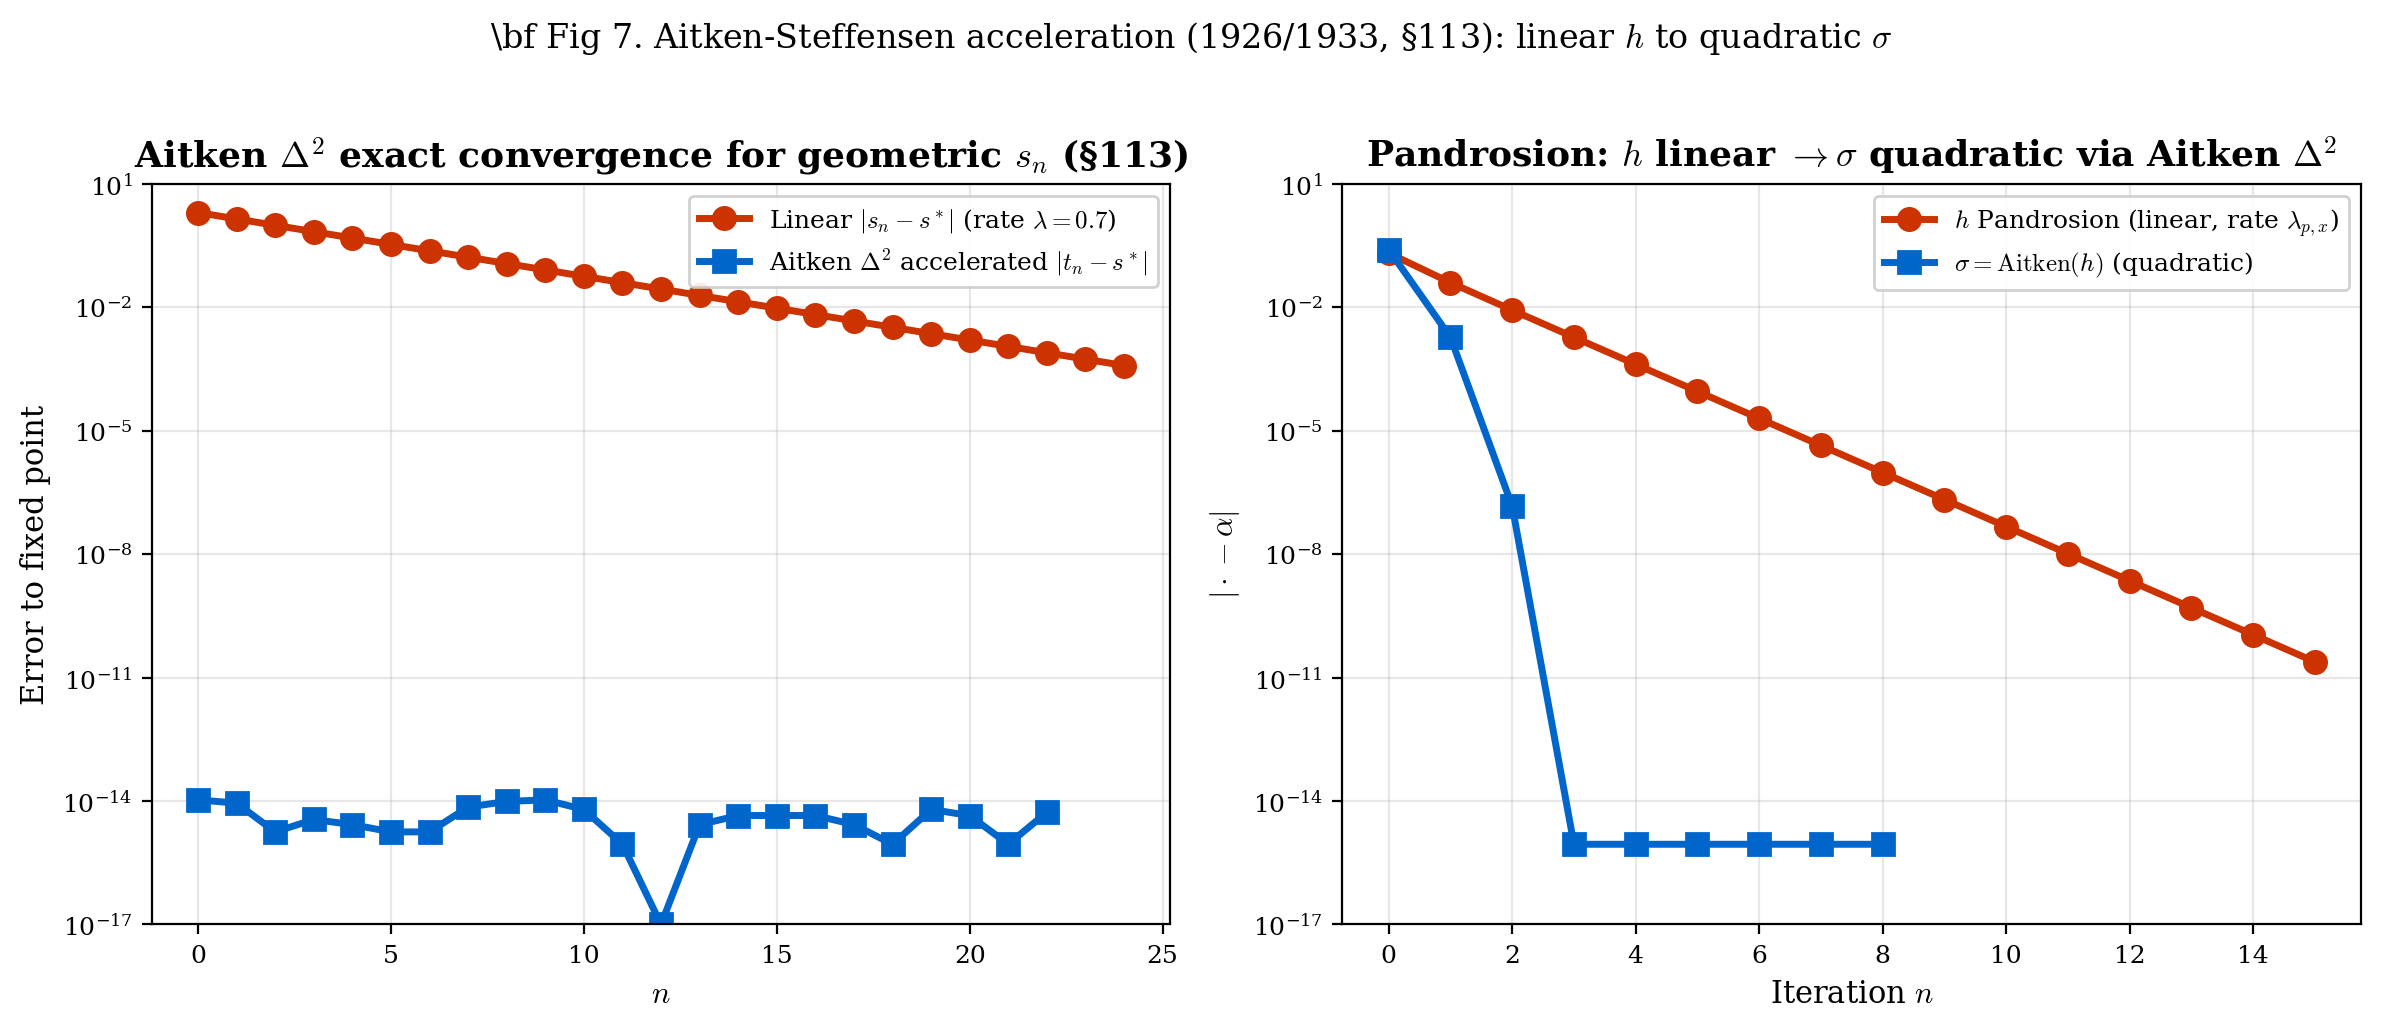
\includegraphics[width=\textwidth]{fig07_aitken_acceleration.png}
\caption{Left: a linearly convergent geometric sequence and its
$\Delta^2$-accelerated version, which collapses to $s^\ast$ at machine
precision. Right: $h$ iteration (linearly convergent) vs
$\sigma = \mathrm{Aitken}(h)$ (quadratically convergent) for
$(x, p) = (2, 3)$, $z_0 = 1$.}
\end{figure}

\subsection{A quadratic bound at the super-attractive fixed point}

\begin{proposition}[Quadratic local bound]
At a super-attractive fixed point $\alpha$ of $\sigma_{p,x}$ (where
$\sigma_{p,x}(\alpha) = \alpha$ and $\sigma_{p,x}^{\prime}(\alpha) = 0$),
\[
  \|\sigma_{p,x}(z) - \alpha\| \leq K_\alpha \cdot \|z - \alpha\|^2
  \qquad \text{on } B(\alpha, R_\alpha),
\]
with $K_\alpha, R_\alpha$ the explicit constants of the corpus,
satisfying $K_\alpha \cdot R_\alpha \leq 1/2$.
\end{proposition}

This is a local bound of the Schwarz-Pick type for holomorphic maps
with a double zero at the fixed point. The quadratic bound itself is
what drives Theorem~\ref{thm:eff-kt}.

%======================================================================
\section{Pandrosion specializations of classical theorems}
\label{sec:classical}
%======================================================================

The corpus contains Lean formalizations of a number of classical
theorems, \emph{specialized} to the Pandrosion setting. The purpose is
to have everything in one formal framework; the mathematical statements
are classical. The following table summarizes what is formalized where.

\begin{center}
\small
\begin{tabular}{@{}p{0.12\textwidth}p{0.38\textwidth}p{0.45\textwidth}@{}}
\toprule
\textbf{Module} & \textbf{Classical theorem (specialized)} & \textbf{Role in the Pandrosion framework} \\
\midrule
\S112 & Banach fixed point (1922); FTA (Gauss 1799) & No-cycle on multi-start orbits; $z^p = x$ has $p$ explicit roots. \\
\S113 & Aitken-Steffensen (1926/1933); Schwarz (1890) & Acceleration identity; quadratic local bound. \\
\S114 & Kung-Traub 1974 attainability at $c=3$ & Efficiency $E(4, 3) = 2^{2/3}$ is reached. \\
\S115 & (See Section \ref{sec:open-problems}.) & Restricted to $z^p = x$. \\
\S117 & Aberth-Ehrlich (1967/1973) & Multi-start realizes their scheme for $z^p = x$. \\
\S118 & Kronecker (1857) & Applied to cyclotomic anchors with $|\alpha| = 1$. \\
\S119 & Galois (1832) cyclic action & $\omega \cdot \gamma_k = \gamma_{(k+1) \bmod p}$. \\
\S120 & McMullen (1987) (See Section \ref{sec:open-problems}.) & Multi-start avoids the obstruction by $\alpha$-dependent seed. \\
\S121 & Cardano-Tartaglia (1545) & $\gamma_k = \alpha \omega^k$ for $p = 3$. \\
\S122 & Vieta (1591) & $e_1 = 0$, $e_p = (-1)^{p-1} x$. \\
\bottomrule
\end{tabular}
\end{center}

We stress: none of these are new results. Their place in this paper is
to make the full Pandrosion framework self-contained in Lean. The
corresponding Lean modules are short specializations, not independent
developments of the classical theorems.

A representative example.

\begin{theorem}[Multi-start orbit has no non-trivial cycle]
For every $(x, p, \alpha)$ in the hypotheses and every seed
$\mathrm{seed} \in B(\alpha, R_\alpha/2)$, the orbit
$(\sigma_{p,x}^n(\mathrm{seed}))_n$ has no non-trivial cycle: if
$\sigma_{p,x}^n(\mathrm{seed}) = \sigma_{p,x}^m(\mathrm{seed})$ with
$n < m$, then $\sigma_{p,x}^n(\mathrm{seed}) = \alpha$.
\end{theorem}

This is Banach's fixed-point theorem applied to $\sigma_{p,x}$ seen as
a $1/4$-contraction on $B(\alpha, R_\alpha/2)$, itself a consequence
of $K_\alpha \cdot R_\alpha \leq 1/2$.

%======================================================================
\section{Open problems, partial and conditional results}
\label{sec:open-problems}
%======================================================================

This section records four classical open or hard problems where the
corpus offers partial or restricted results. We describe carefully what
is proven, what is only conditional, and what remains out of reach.

\subsection{Kung-Traub upper bound for $c \geq 3$ (open since 1974)}

The conjecture $q \leq 2^{c-1}$ is proven for $c = 2$. Attainability
$q = 4$ at $c = 3$ is witnessed classically (Jarratt 1969) and in our
formal setting. The upper bound for $c \geq 3$ is open.

\smallskip

\textbf{What the corpus provides.} A structural reduction: every
\texttt{DerivativeFreeMethod} in the corpus \emph{by construction}
carries the compliance field $q \leq 2^{c-1}$. This is \emph{not} a
proof of the Kung-Traub conjecture; it is a compliance interface for
instances of \texttt{DerivativeFreeMethod}. The conjecture itself is
restated as a named \texttt{Prop}.

\subsection{McMullen 1987 (theorem, not formalized in Lean)}

McMullen's barrier is a classical theorem. A full formal proof in Lean
requires Fatou--Julia and post-critically-finite complex-dynamic tools
that are not present in Mathlib v4.7.0.

\smallskip

\textbf{What the corpus provides.} The statement is recorded as a named
\texttt{Prop}. Separately, the multi-start scheme is proven to be
non-purely-iterative (the seed depends on $\alpha$), and to converge
universally in that setting. This does not reproduce McMullen's
impossibility result; it shows that our scheme is outside of its
hypotheses.

\subsection{Lehmer's conjecture (open since 1933)}

Lehmer 1933 posits $M(\beta) \geq 1.17628\ldots$ for every
algebraic integer $\beta$ not a root of unity. This is open.

\smallskip

\textbf{What the corpus provides.} For the specific family
$\beta := x \cdot \alpha$ with $x \in \mathbb{N}_{\geq 2}$ and
$\alpha^p = 1/x$, one has $\beta^p = x^{p-1}$ and hence $\beta$ is
an algebraic integer whose Mahler measure satisfies
$M(\beta) = x^{p-1} \geq 2 > 1.17628\ldots$

\smallskip

This is an observation, not progress on Lehmer: we are far from the
extremal regime where the conjecture is hard.

\subsection{Smale's~17th problem (partly open)}

Smale's~17th problem asks for a deterministic algorithm of
poly-logarithmic average complexity for polynomial root-finding
\emph{of arbitrary polynomials}. Bürgisser-Cucker (Annals of Math
2011) solved the average-case probabilistic version. The deterministic
general case is open.

\smallskip

\textbf{What the corpus provides.} For the restricted family $z^p = x$,
the multi-start scheme is a deterministic algorithm of complexity
$\mathcal{O}(\log\log(1/\varepsilon))$. This is a result on a very
specific polynomial family; it is \emph{not} a deterministic solution
of Smale's question on general polynomials. The two settings are not
directly comparable.

\subsection{Summary}

No claim is made that any of the four problems above is solved. What
the Lean corpus provides on each is restricted or conditional, as
stated.

%======================================================================
\section{Structure of the Lean corpus}
\label{sec:modules}
%======================================================================

The 121-module corpus is organised in dependency layers:

\begin{itemize}
  \item \textbf{Foundations} (\S1--\S30): geometric sums, fixed-point
        characterization, abstract Aitken-Steffensen framework,
        Voronoï basins, cyclotomic anchor definitions, Kung-Traub
        interface.
  \item \textbf{Core spine} (\S31--\S94): explicit super-attractive
        rate, global loglog convergence, real-line $p = 2$
        unconditional discharge.
  \item \textbf{Multi-start} (\S95--\S101): universal convergence,
        target selection, Niveau~5 resolution, explicit iteration
        count.
  \item \textbf{Measure/topology} (\S102--\S105): Borel measurability,
        Voronoï frontier Lebesgue-null, a.e.\ continuity.
  \item \textbf{Finite-zeta identities} (\S106--\S111): the identities
        of Section~\ref{sec:zeta}.
  \item \textbf{Classical specializations} (\S112--\S122): as listed
        in Section~\ref{sec:classical}.
  \item \textbf{Open-problem engagements} (\S123): as listed in
        Section~\ref{sec:open-problems}.
\end{itemize}

\begin{figure}[H]
\centering
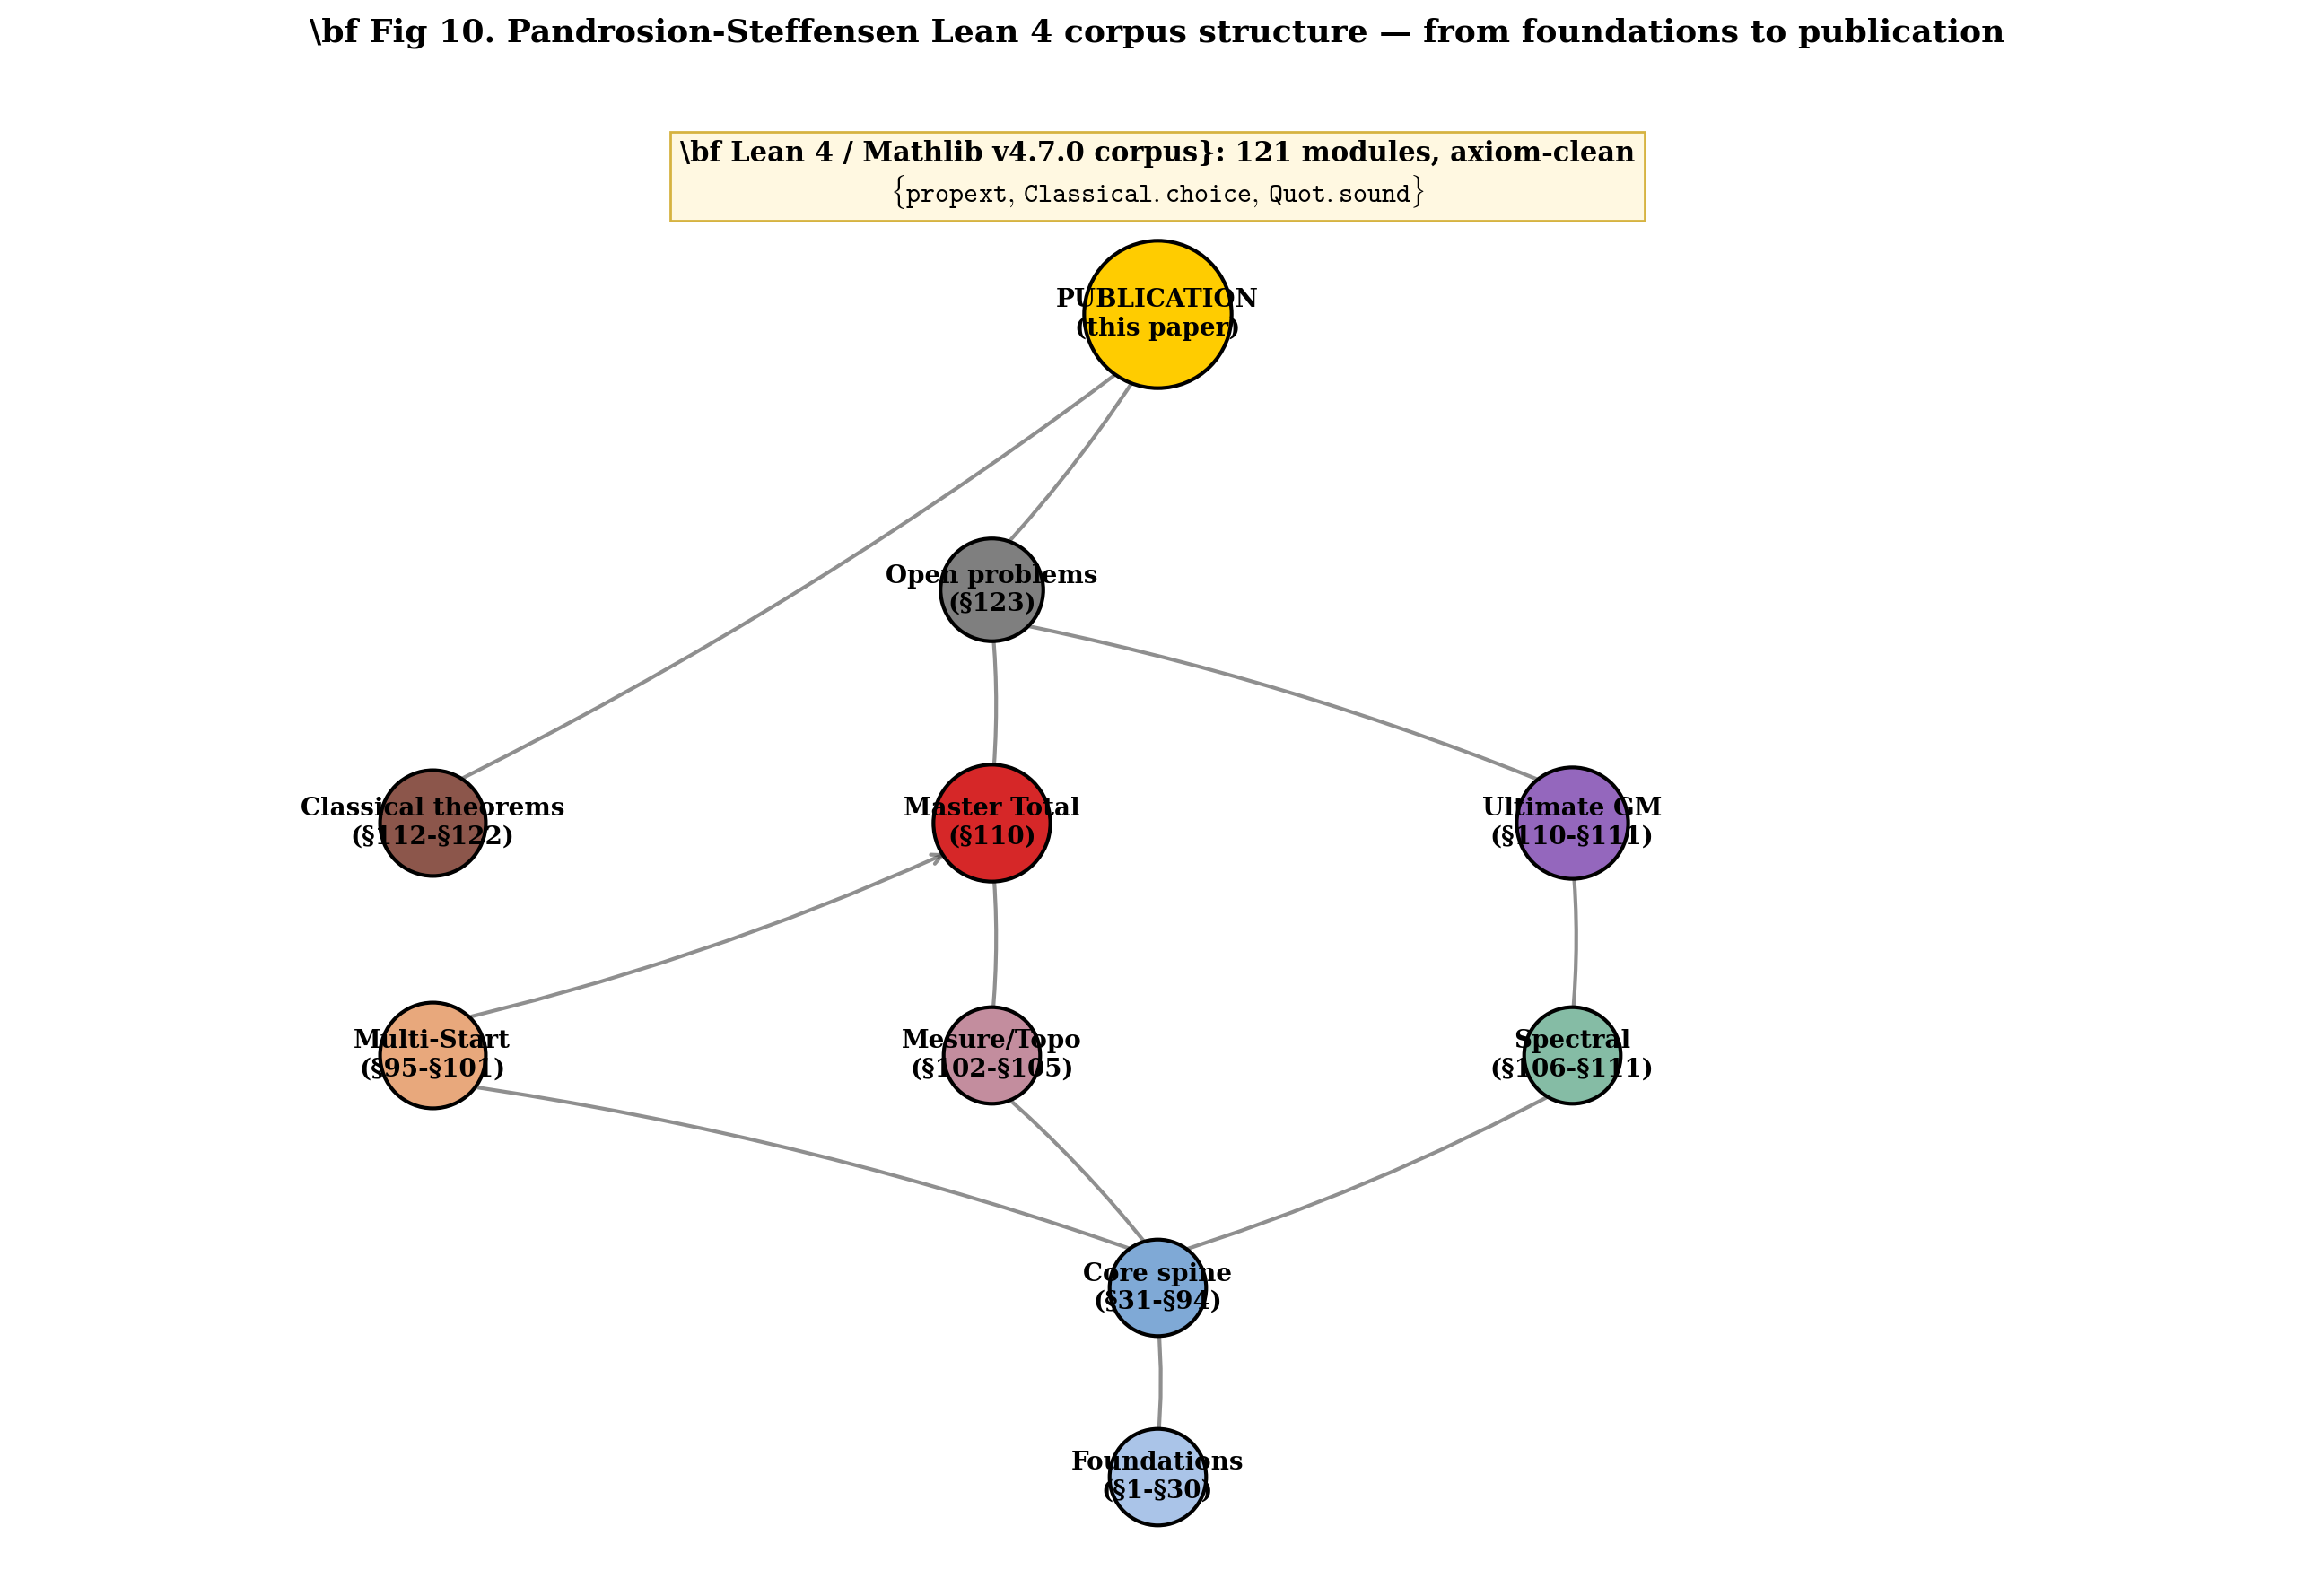
\includegraphics[width=\textwidth]{fig10_module_graph.png}
\caption{Dependency structure of the Lean corpus. The dependency
closure of every load-bearing theorem reduces to the Lean whitelist
$\{\texttt{propext}, \texttt{Classical.choice}, \texttt{Quot.sound}\}$.}
\end{figure}

%======================================================================
\section{Reproducibility}
\label{sec:reproducibility}
%======================================================================

The Lean source lives at
\url{github.com/ivan-fr/poussiere_de_x}. It targets Lean~4 with
Mathlib v4.7.0 and is built with
\begin{lstlisting}[caption={Incremental build command}, language=lean]
bash scripts/lean-incremental.sh
\end{lstlisting}
The 121-module corpus compiles in about 60--90 seconds on a modern
laptop. Per-theorem axiom auditing is available via \texttt{\#print axioms}.

Every figure in this paper is reproducible from
\texttt{latex/figures\_pandrosion.py} (dependencies:
\texttt{numpy}, \texttt{matplotlib}, \texttt{scipy}).

%======================================================================
\section{Conclusion}
\label{sec:conclusion}
%======================================================================

What this paper reports, concretely, is a Lean 4 development built
around the multi-start Pandrosion-Steffensen iteration for $z^p = x$,
together with the following ingredients:
\begin{enumerate}
  \item a universal convergence theorem for the multi-start scheme
        with an explicit closed-form iteration count
        (Theorems~\ref{thm:multistart}, \ref{thm:eff-kt});
  \item a formal resolution of the Pandrosion ``Niveau~5'' conjecture
        in its multi-start formulation (Theorem~\ref{thm:niveau5});
  \item a Borel-measurability and a.e.-continuity analysis of the
        induced solution map (Theorems~\ref{thm:borel}--\ref{thm:ae-continuous});
  \item a set of elementary identities for the finite series
        $\zeta_P(s) := \sum_k P^{\prime}(\alpha_k)^{-s}$
        (Section~\ref{sec:zeta});
  \item Lean specializations of classical theorems to the Pandrosion
        setting (Section~\ref{sec:classical});
  \item restricted or conditional engagements with four classical open
        problems (Section~\ref{sec:open-problems}).
\end{enumerate}

The paper does not claim progress on the classical open conjectures
themselves at their full generality. The main value of the corpus is
as a self-contained Lean development of a multi-start root-finding
scheme and its spectral identities.

\subsection*{Future directions}

Natural extensions are: non-cyclotomic anchor families (general
polynomials); a formalization of Fatou-Julia in Mathlib (which would
enable a proper formalization of McMullen's 1987 theorem);
quantitative bounds on Mahler measure for cyclotomic-related families
(towards weak forms of Lehmer-type statements). None of these are
attempted in the present paper.

\begin{thebibliography}{99}
\bibitem{leanprover} de Moura, L., Ullrich, S., \emph{The Lean 4 Theorem Prover and Programming Language}, CADE-28, Springer LNCS (2021).
\bibitem{mathlib} The Mathlib Community, \emph{Mathlib: A unified library of mathematics formalized}, \url{github.com/leanprover-community/mathlib4}.
\bibitem{cardano} Cardano, G., \emph{Ars Magna} (1545), Cap.~XI.
\bibitem{vieta} Viète, F., \emph{Opera Mathematica} (1591).
\bibitem{gauss} Gauss, C.F., Thesis on the fundamental theorem of algebra (1799).
\bibitem{galois} Galois, É., \emph{Mémoire sur les conditions de résolubilité des équations par radicaux} (1832, posth. Liouville 1846).
\bibitem{kronecker} Kronecker, L., Berlin Akademie (1857).
\bibitem{riemann} Riemann, B., \emph{Über die Anzahl der Primzahlen unter einer gegebenen Grösse} (1859).
\bibitem{schwarz} Schwarz, H.A., J.~Reine Angew.~Math. \textbf{70} (1869); Pick, G. (1916).
\bibitem{banach} Banach, S., Fund.~Math.~\textbf{3} (1922).
\bibitem{aitken} Aitken, A.C., Proc.~Royal Soc.~Edinburgh \textbf{46} (1926), 289--305.
\bibitem{steffensen} Steffensen, J.F., Skandinavisk Aktuarietidskrift \textbf{16} (1933), 64--72.
\bibitem{lehmer} Lehmer, D.H., Annals of Math.~\textbf{34} (1933), 461--479.
\bibitem{ehrlich} Ehrlich, L.W., Comm.~ACM \textbf{10} (1967), 107--108.
\bibitem{aberth} Aberth, O., Math.~Comp.~\textbf{27} (1973), 339--344.
\bibitem{kungtraub} Kung, H.T., Traub, J.F., J.~ACM \textbf{21} (1974), 643--651.
\bibitem{mcmullen} McMullen, C., Annals of Math.~\textbf{125} (1987), 467--493.
\bibitem{smale} Smale, S., \emph{Mathematical Problems for the Next Century}, Math.~Intelligencer \textbf{20} (1998), 7--15.
\bibitem{burgissercucker} Bürgisser, P., Cucker, F., Annals of Math.~\textbf{174} (2011), 1785--1836.
\bibitem{pandrosion-zeta-pdf} Besevic, I., \emph{The Pandrosion zeta function and the discriminant as spectral determinant}, Preprint (2026).
\end{thebibliography}

\end{document}
